\section{Test Beam Setup}


The new readout modules being installed in the CMS detector have several new components such as new charge integrator and encoder (QIE) chips~\cite{QIE, QIE2}, but the main subject of my work was the SiPM. To study the features of the SiPM,  such as nonlinearity, we used a test beam. The particles in the beam are at energies from about 10 to 500 GeV, and we can control the energy and types of the particles in the beam. There are several different experiments that use this beam, and the HCAL has a mock test stand that can be moved into the path of the beam when experiments need to be run. The CMS detector is 100 meters underground and is in a cavern that, due to radiation and tight enclosures, makes the detector difficult to access. Though modifications and maintenance can be made during shutdowns, this is not the ideal way to perform tests on new electronics. The test stand at the test beam location called H2 is on ground level and can be easily accessed. In addition, the energy and particle type of the beam can be easily controlled. The test stand is designed to be similar to a portion of the HCAL on CMS. Using this test beam, we can shoot particles such as pions at the test stand, which has the new readout module installed, and look at the response~\cite{TB96, TB06}. We can vary the energy of incident particles, which should increase the number of photons produced in the scintillator tiles. This means there will be more input photons on the SiPMs.

We need to collect a large amount of data in order to measure the features of new readout modules with high statistical accuracy. To achieve this, we take multiple runs with several thousand events or particles hitting the test stand. Because we will be taking data over a long period of time, we want to ensure that we record data only when a particle is hitting the test stand. One of the key systems that helps with this is the trigger system. In the path of the beam before the test stand we put scintillator tiles in order to send a generic signal to the control room. A total of four tiles were placed in the path of the beam. When we see signals from these tiles we know that a particle is coming from the beam. This serves as a trigger signal for our data acquisition system. The trigger signal then goes to the back-end electronics that stores the data from the detector. In this way we only store data around the time when we know a particle is hitting our test stand. There is also a ready signal that goes from the back-end electronics to the trigger. Since a particle may come before the back-end electronics are finished storing the relevant data, a trigger signal that comes without the ready signal will simply be ignored.

\begin{figure}
\centering
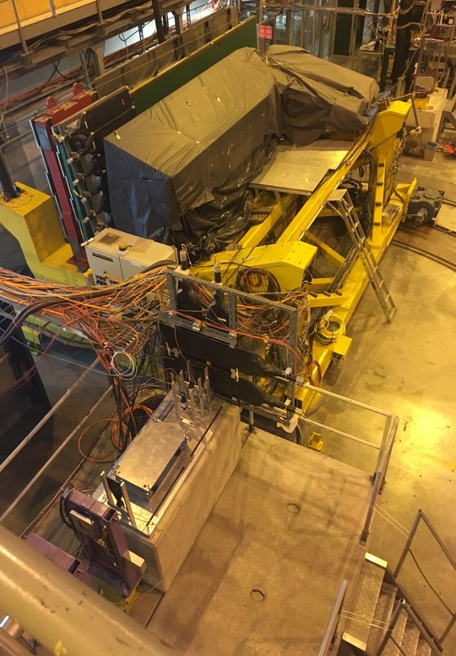
\includegraphics[width=0.6\linewidth]{Figures/Teststand.png}
\caption{The HCAL test stand at H2. The scintillator tiles are covered in black tedlar and the new readout modules are connected in the back. The stand can be shifted so the beam can be aimed at different sections.}
\label{fig:stand}
\end{figure}

Although built to be similar to the HCAL on the CMS detector, the test stand is smaller and has some differences. When looking at the data from the test beam, it is important to be sure that the e-map, which, traces the channels that receive the data to the actual scintillator tiles on the detector, is correct. There are some differences between the mock detector at H2 and the HCAL detector in the CMS cavern. In order to account for these differences, a new emap was created for the test beam setup. With an accurate e-map we can create an accurate picture of the incident particles hitting the test stand. The test beam allows us to control the energy and type of particles incident on the test stand. This allows us to study things such as SiPM nonlinearity as we can look at the output of the SiPMs under $50 \GeV$ pions then increase the energy to $150 \GeV$ and compare the different responses. 

SiPM nonlinearity is not the only thing that is being researched using the test beam. In the test beam, the particles come at a low enough frequency, which allows us to isolate the signal of individual particles. This allows us to extract the pulse shape, which is the shape of the output charge vs.\ time. It is also important to see if the pulse shape changes significantly under different circumstances, for example, at higher or lower energies. The well-measured pulse shape of individual signals is necessary information, since it is a vital input to the energy determination of individual incident particles in the CMS detector. Proton collisions occur every 25~ns under nominal LHC conditions; therefore, signals originating from subsequent proton collisions can overlap in time. The pulse shape information is used to resolve the overlapping signals in the CMS detector.

\section{Test Beam Analysis}

With a proper e-map, we can get a picture of the incident particle; we can see its path and where it deposited its energy. Since a particle does not deposit all of its energy in a single scintillator tile, this is critical when reconstructing the particle's energy from multiple neighboring channels. It is also important that there are often a variable amount of scintillator tiles in a single depth channel as shown in Figure~\ref{fig:emap}, which shows 4 scintillator tiles in depth 5 and 3 scintillator tiles in depth 4. It explains why there is more energy deposited in depth 5 rather than depth 4. 

\begin{figure}
\centering
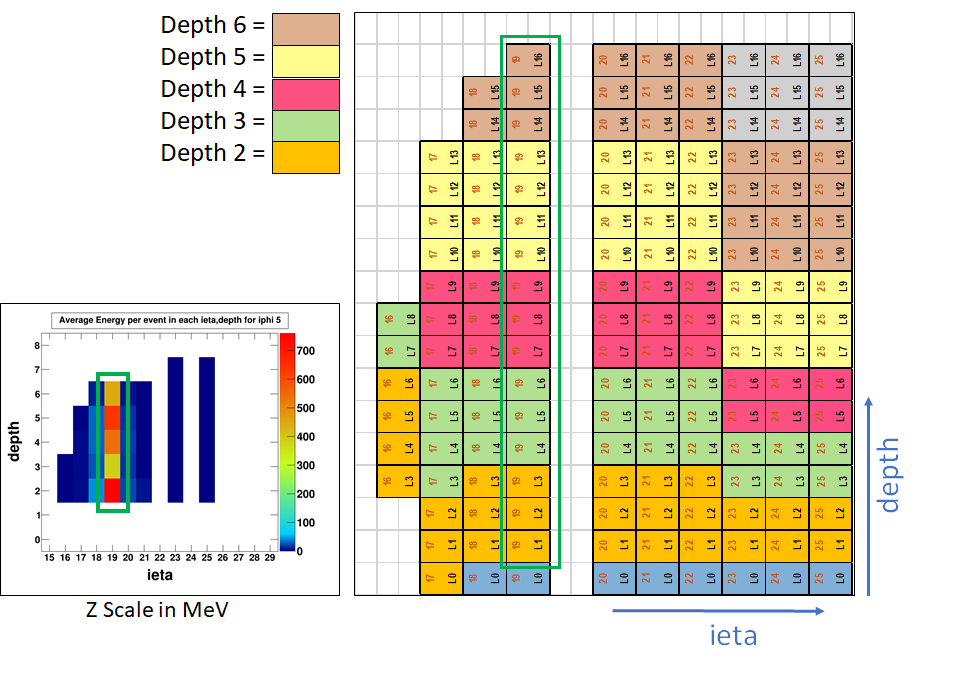
\includegraphics[width=\linewidth]{Figures/eplot.png}
\caption{The emap for a iphi slice of the test stand on the right, which was used to create the figure on the left showing the different places the 150\GeV\space muons deposited energy in the test stand.}
\label{fig:emap}
\end{figure}

Muons are useful for many things, but when trying to reconstruct the energy of particles, it is easier to use pions. The reason for this is that muons tend to go through the detector depositing a small portion of their energy and not being entirely stopped. This can be seen in Figure~\ref{fig:emap}, which shows the muons depositing a nearly constant amount of energy in each of the depths, even the ones further along in the beam's path. Figure~\ref{fig:Muon} shows that the majority of the events in this muon run produced several hundred fC in a single channel of the detector. Trying to reconstruct the energy of the incident muon would not give the actual energy, which would be significantly less than the actual energy of 150\GeV. On the other hand, Figure~\ref{fig:pionmap} shows a plot with a pion run. This shows that the pions deposit a large portion of their energy in the scintillator tiles of depth 2 and deposit less and less in the subsequent depths, with basically nothing in the last depth. There is also a more significant spread in energy compared to the signals in the muon run, which show the muons going straight through while the pions leave some energy in the neighboring channels.

\begin{figure}
\centering
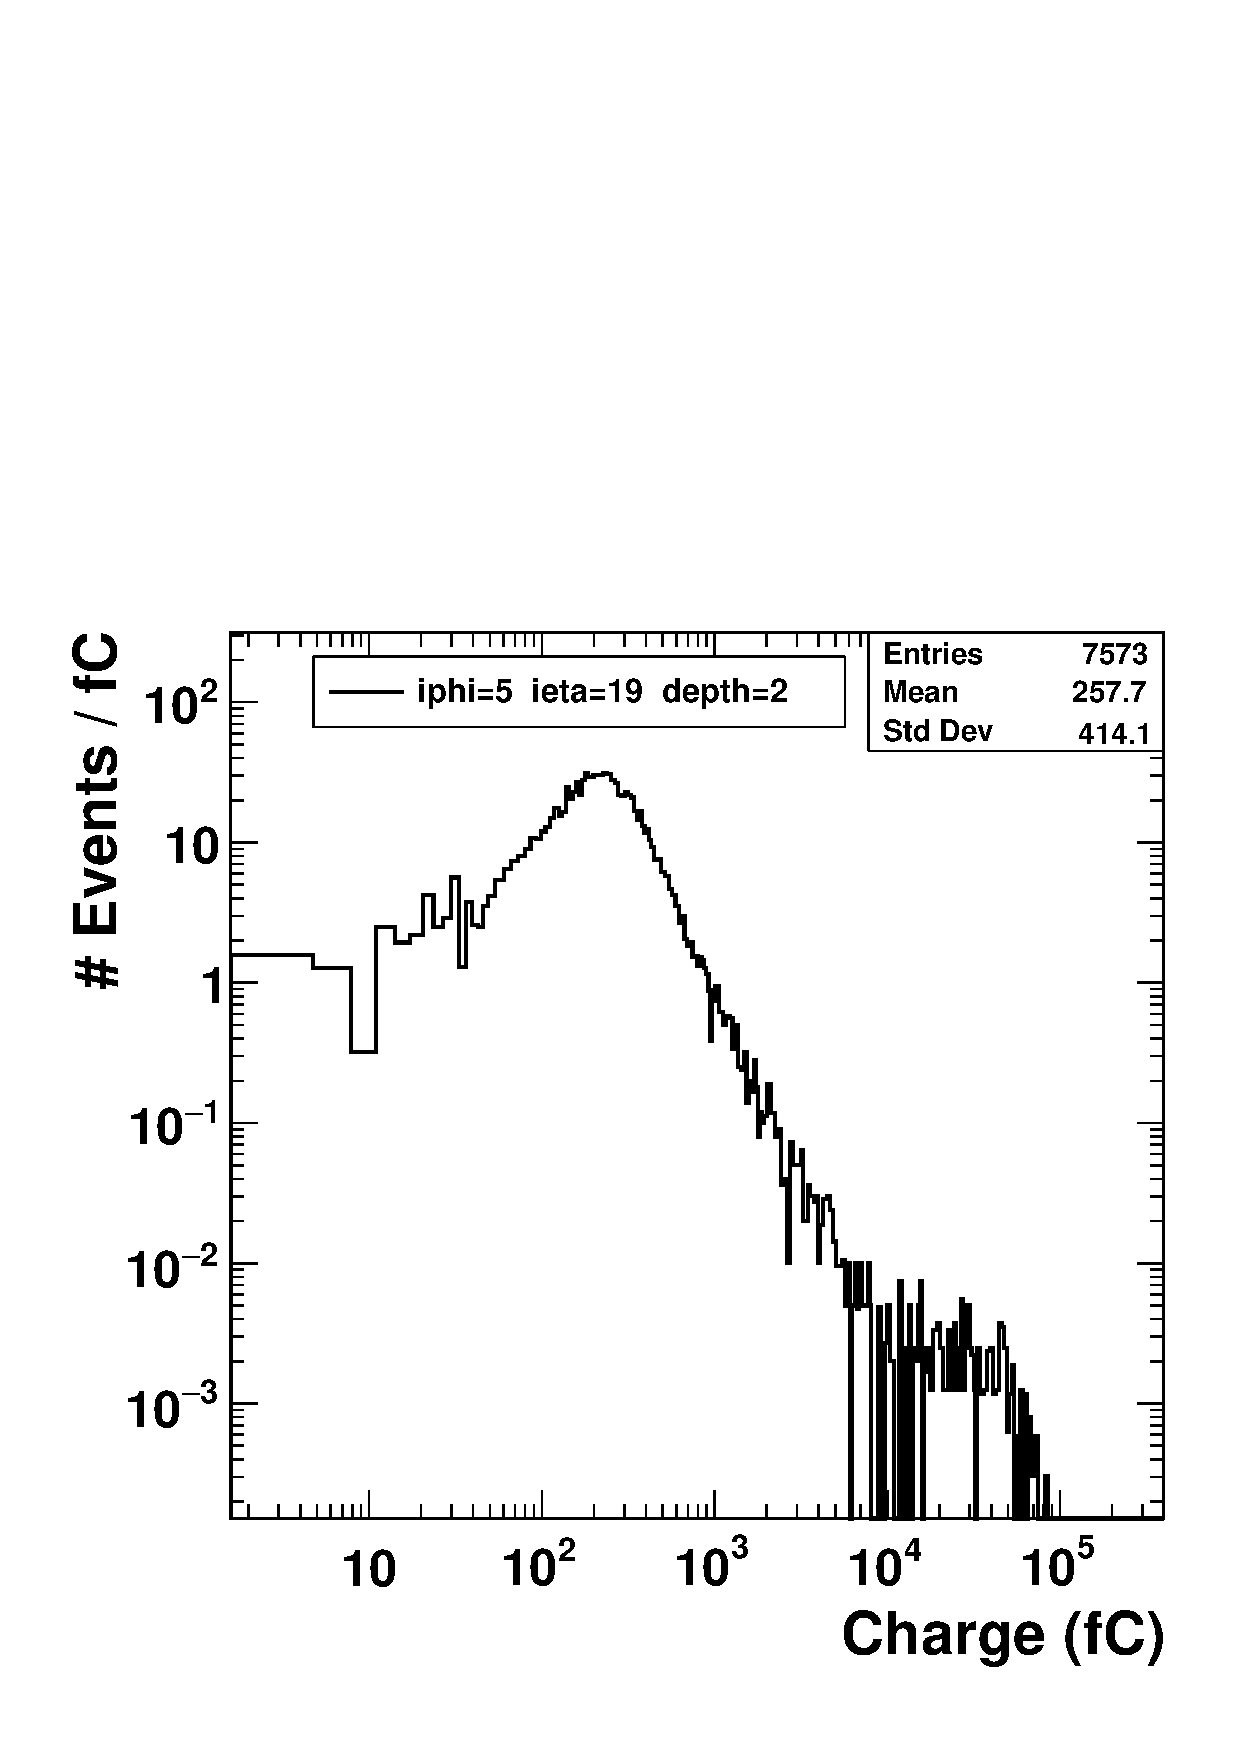
\includegraphics[width=0.7\linewidth]{Figures/MuonCharge.pdf}
\caption{Charge distribution for a single channel (ieta=19, iphi=5, and depth=2) in a 150\GeV\space muon run. The beam in this run was aimed at ieta=19 and iphi=5.}
\label{fig:Muon}
\end{figure}

\begin{figure}
\centering
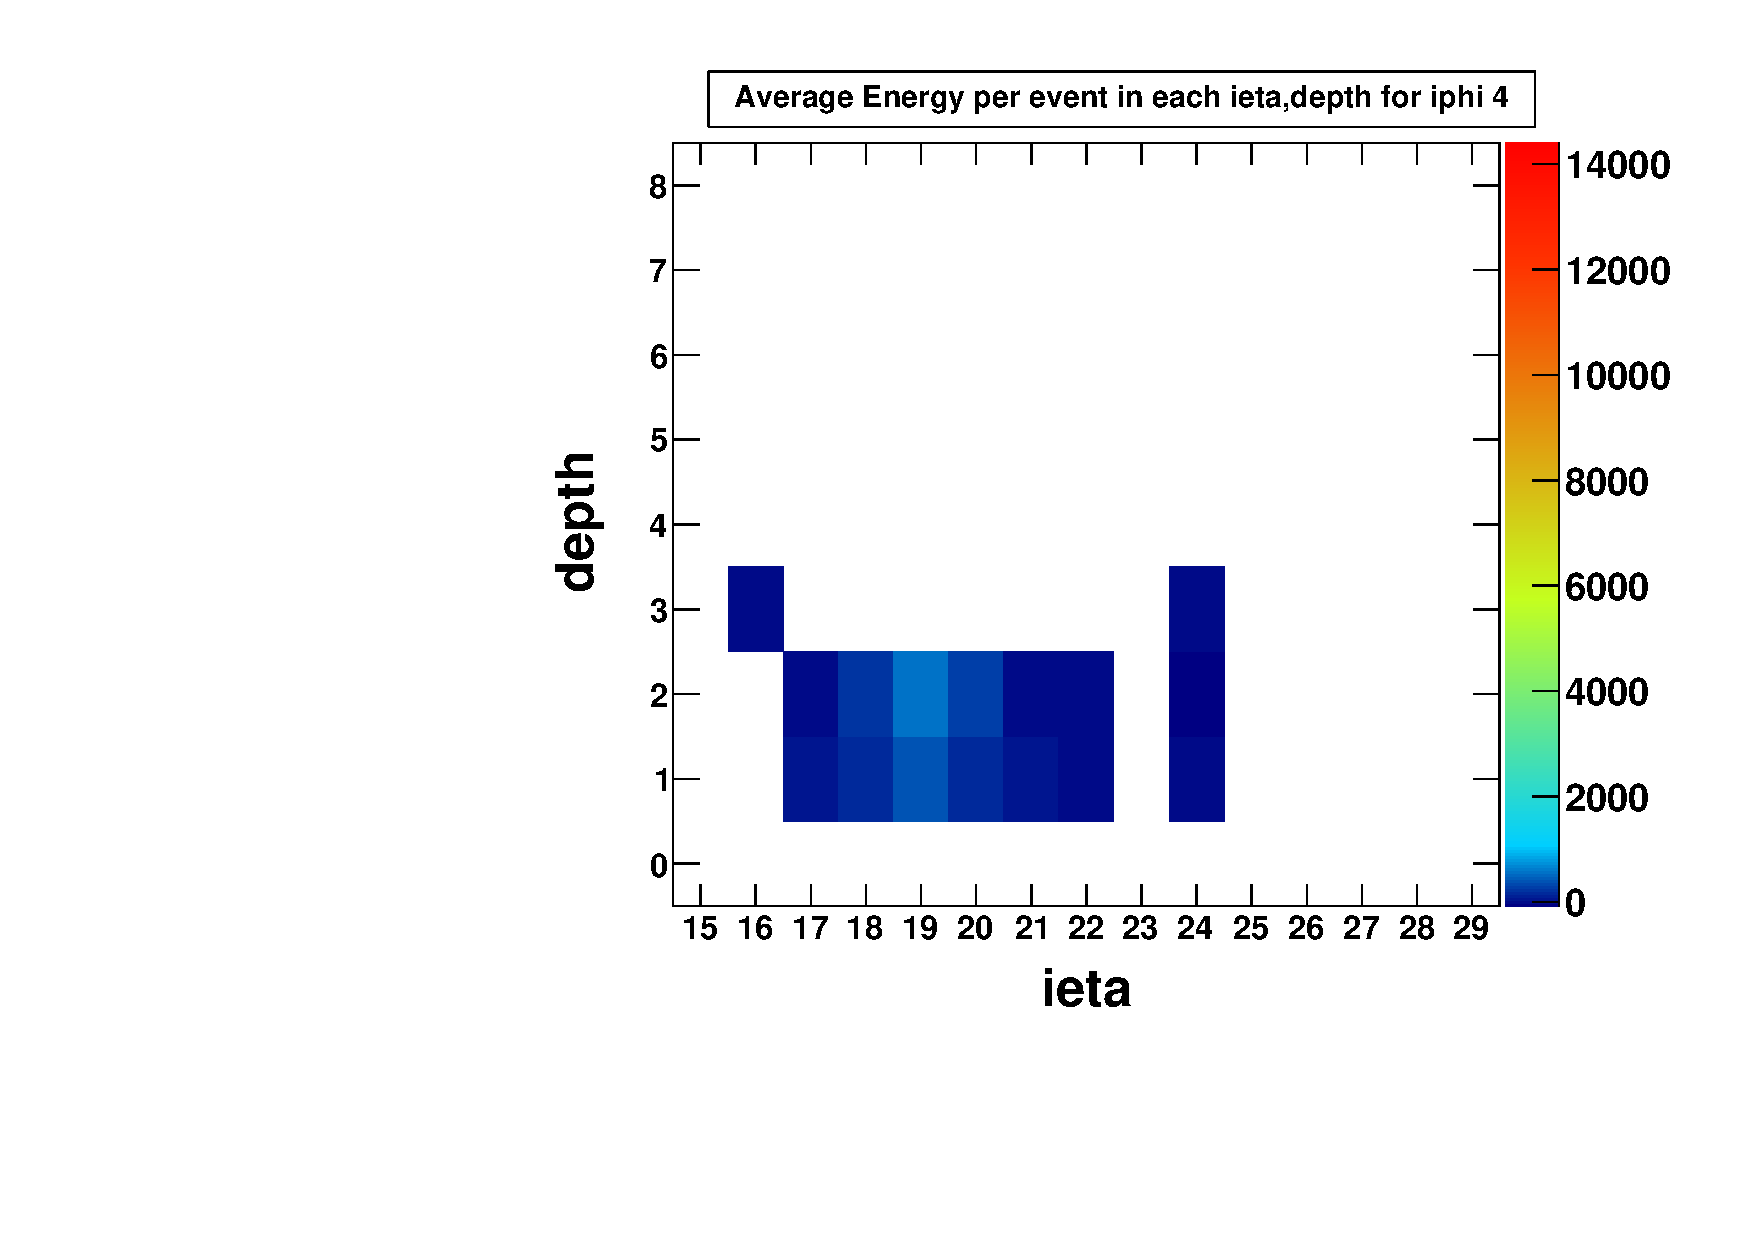
\includegraphics[width=0.495\linewidth]{Figures/pionrun1.pdf}
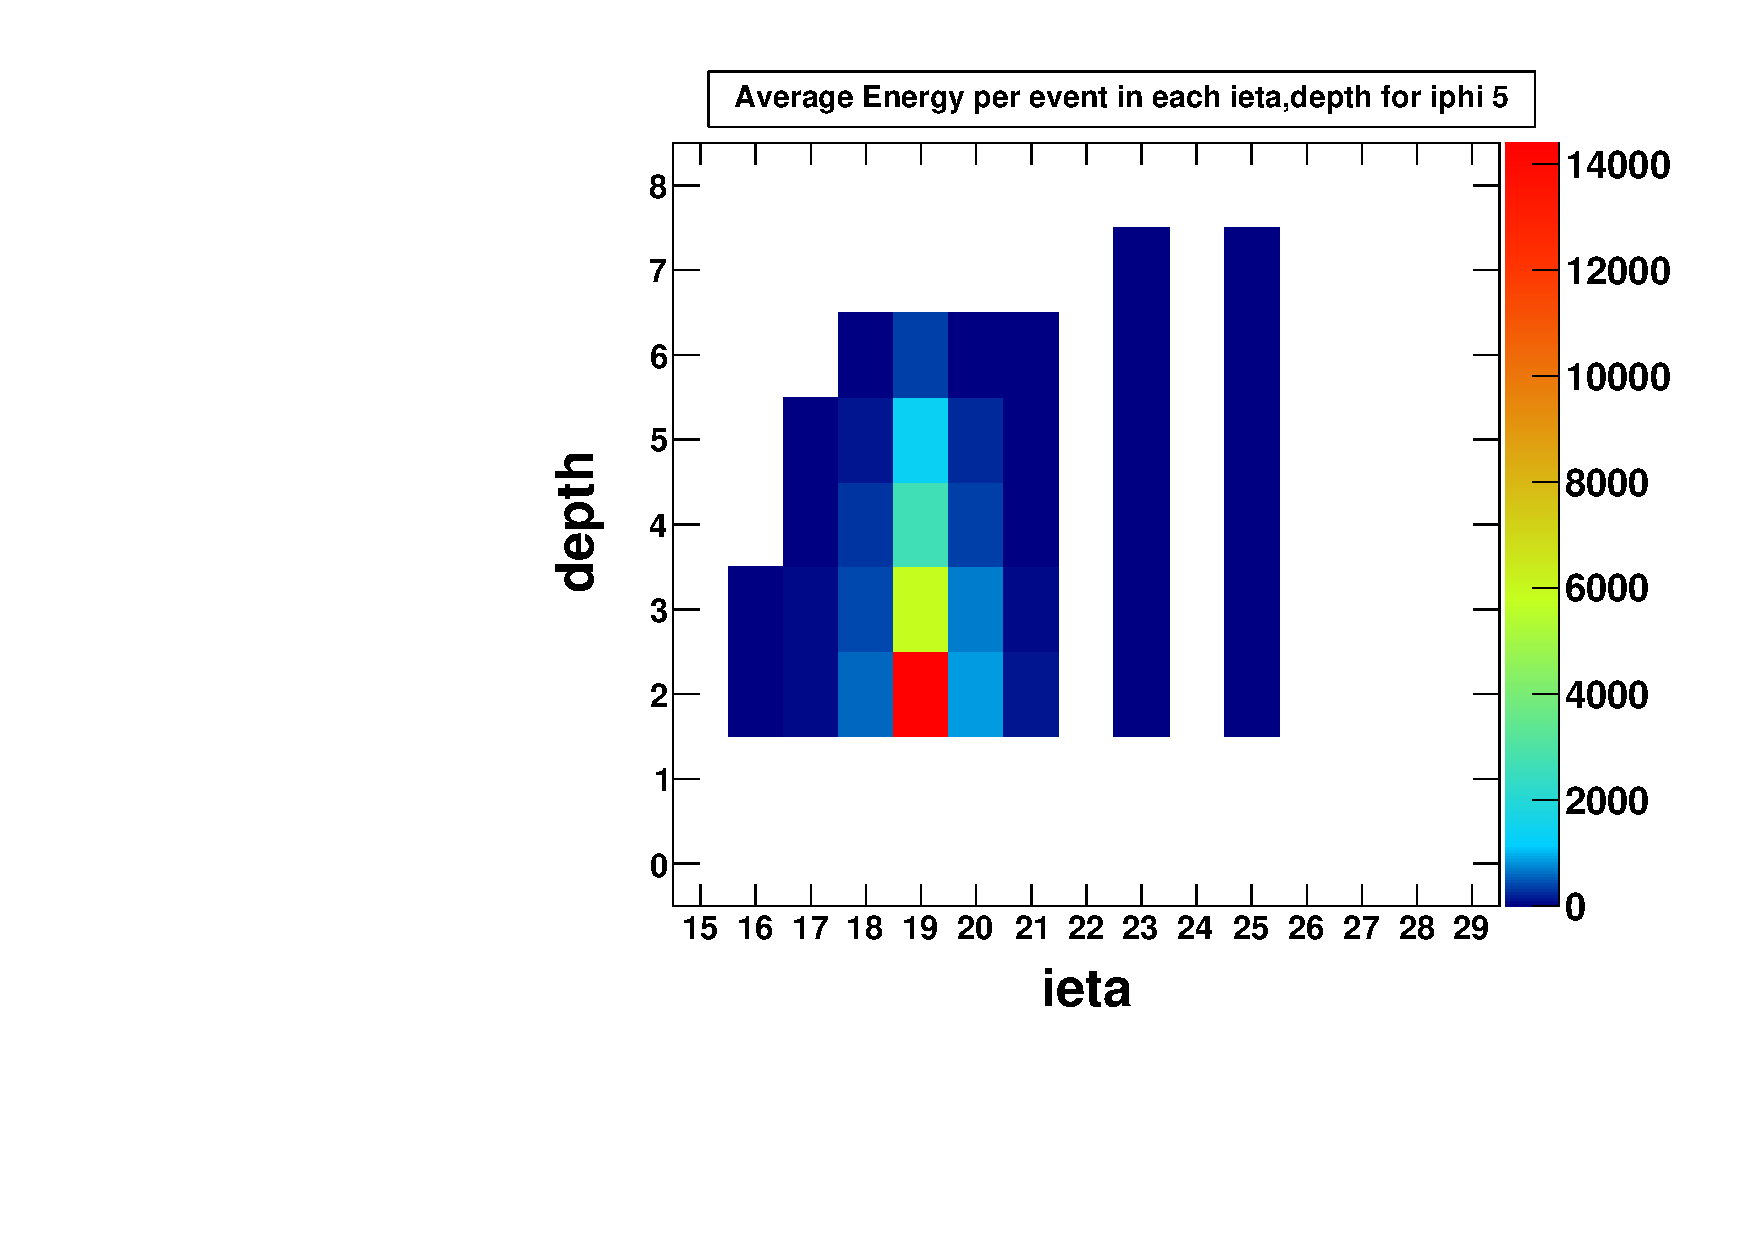
\includegraphics[width=0.495\linewidth]{Figures/pionrun.pdf}
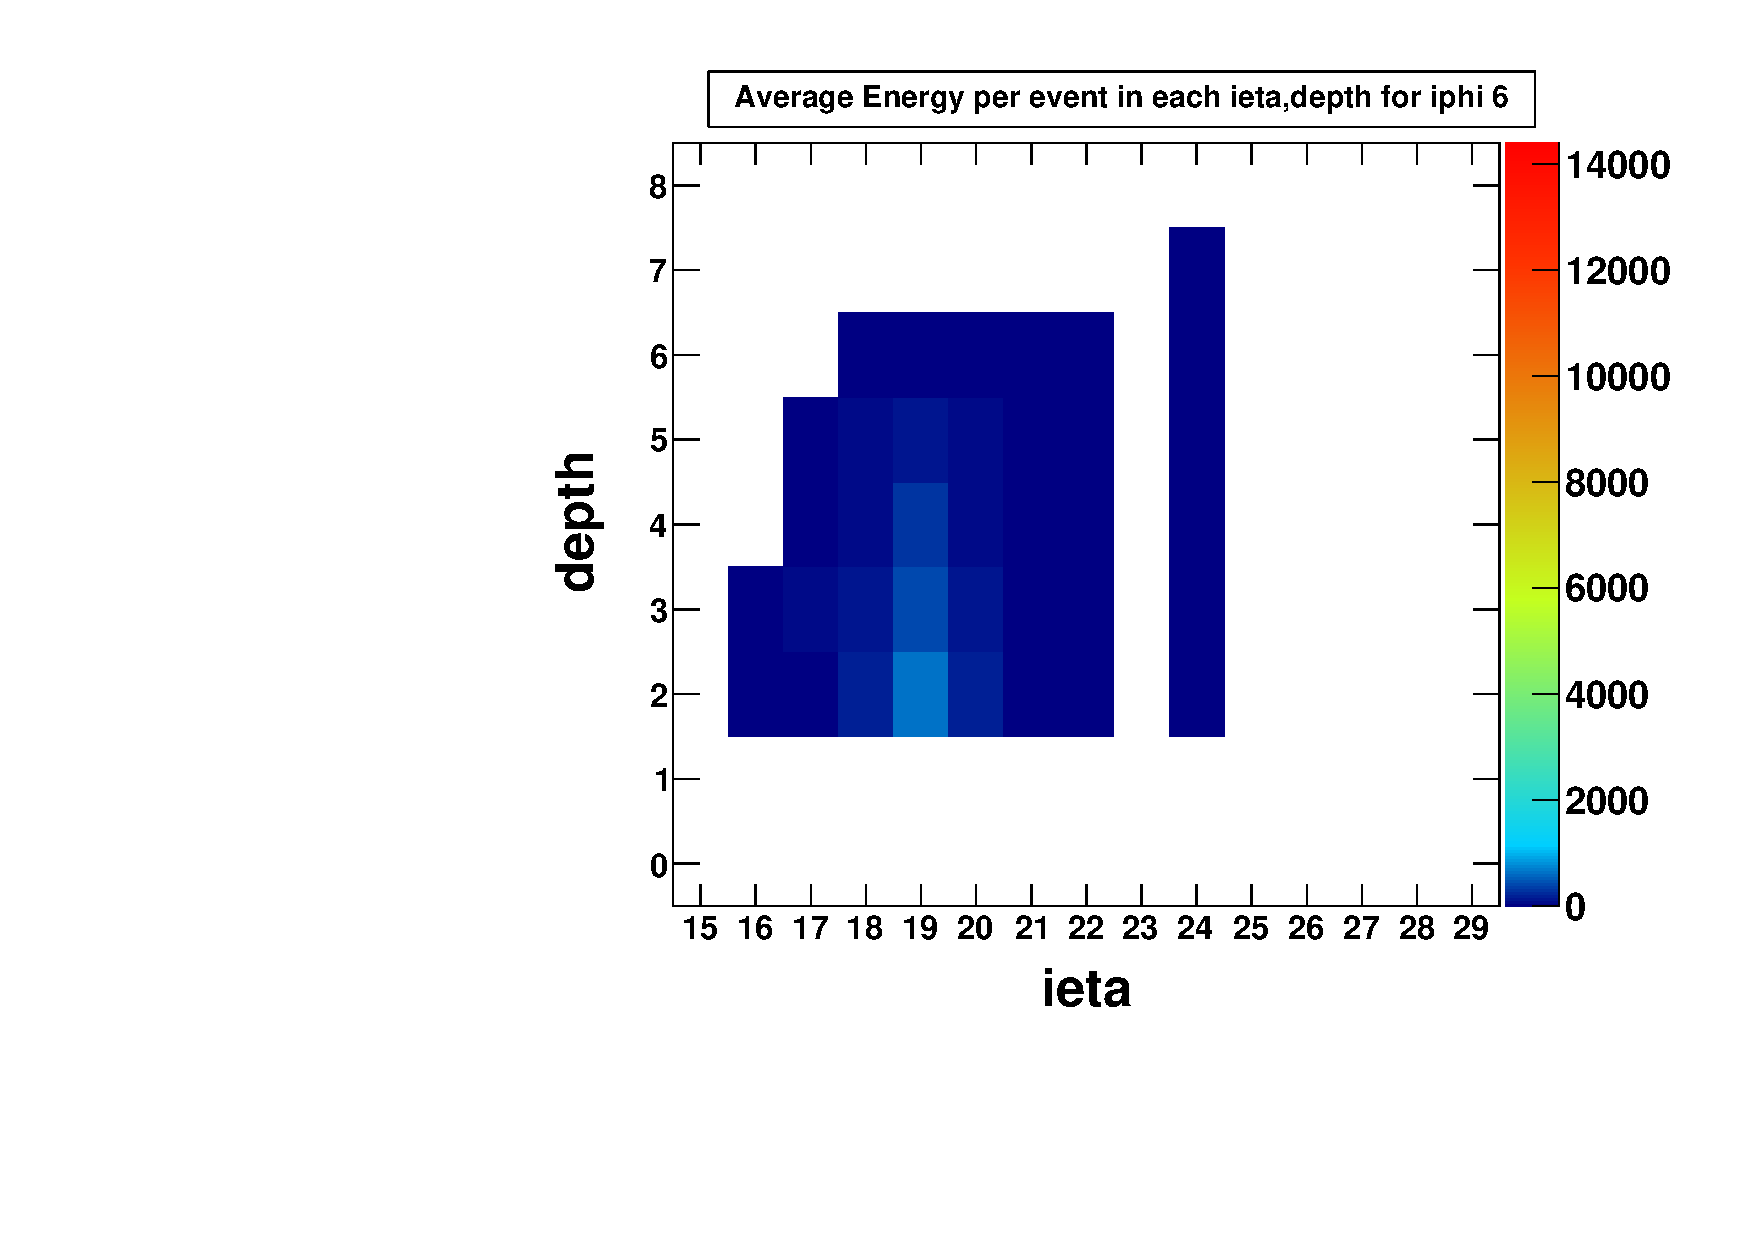
\includegraphics[width=0.495\linewidth]{Figures/pionrun2.pdf}
\caption{Average energy deposited (in \MeV) in the channels in the test beam during a 50\GeV\space pion run aimed at ieta=19 and iphi=5. The different plots show the different iphi locations.}
\label{fig:pionmap}
\end{figure}

To reconstruct the energy of the incident particle we can look at plots such as those in Figure~\ref{fig:pioncharge}, which shows the mean output charge in a 50\GeV\space pion run. By looking at this output charge and the output charge of the other channels, we can find what portion of the particles' energy was deposited in this incident channel and then going by the known energy of the particle how much energy was deposited to produce this output charge. 

\begin{figure}
\centering
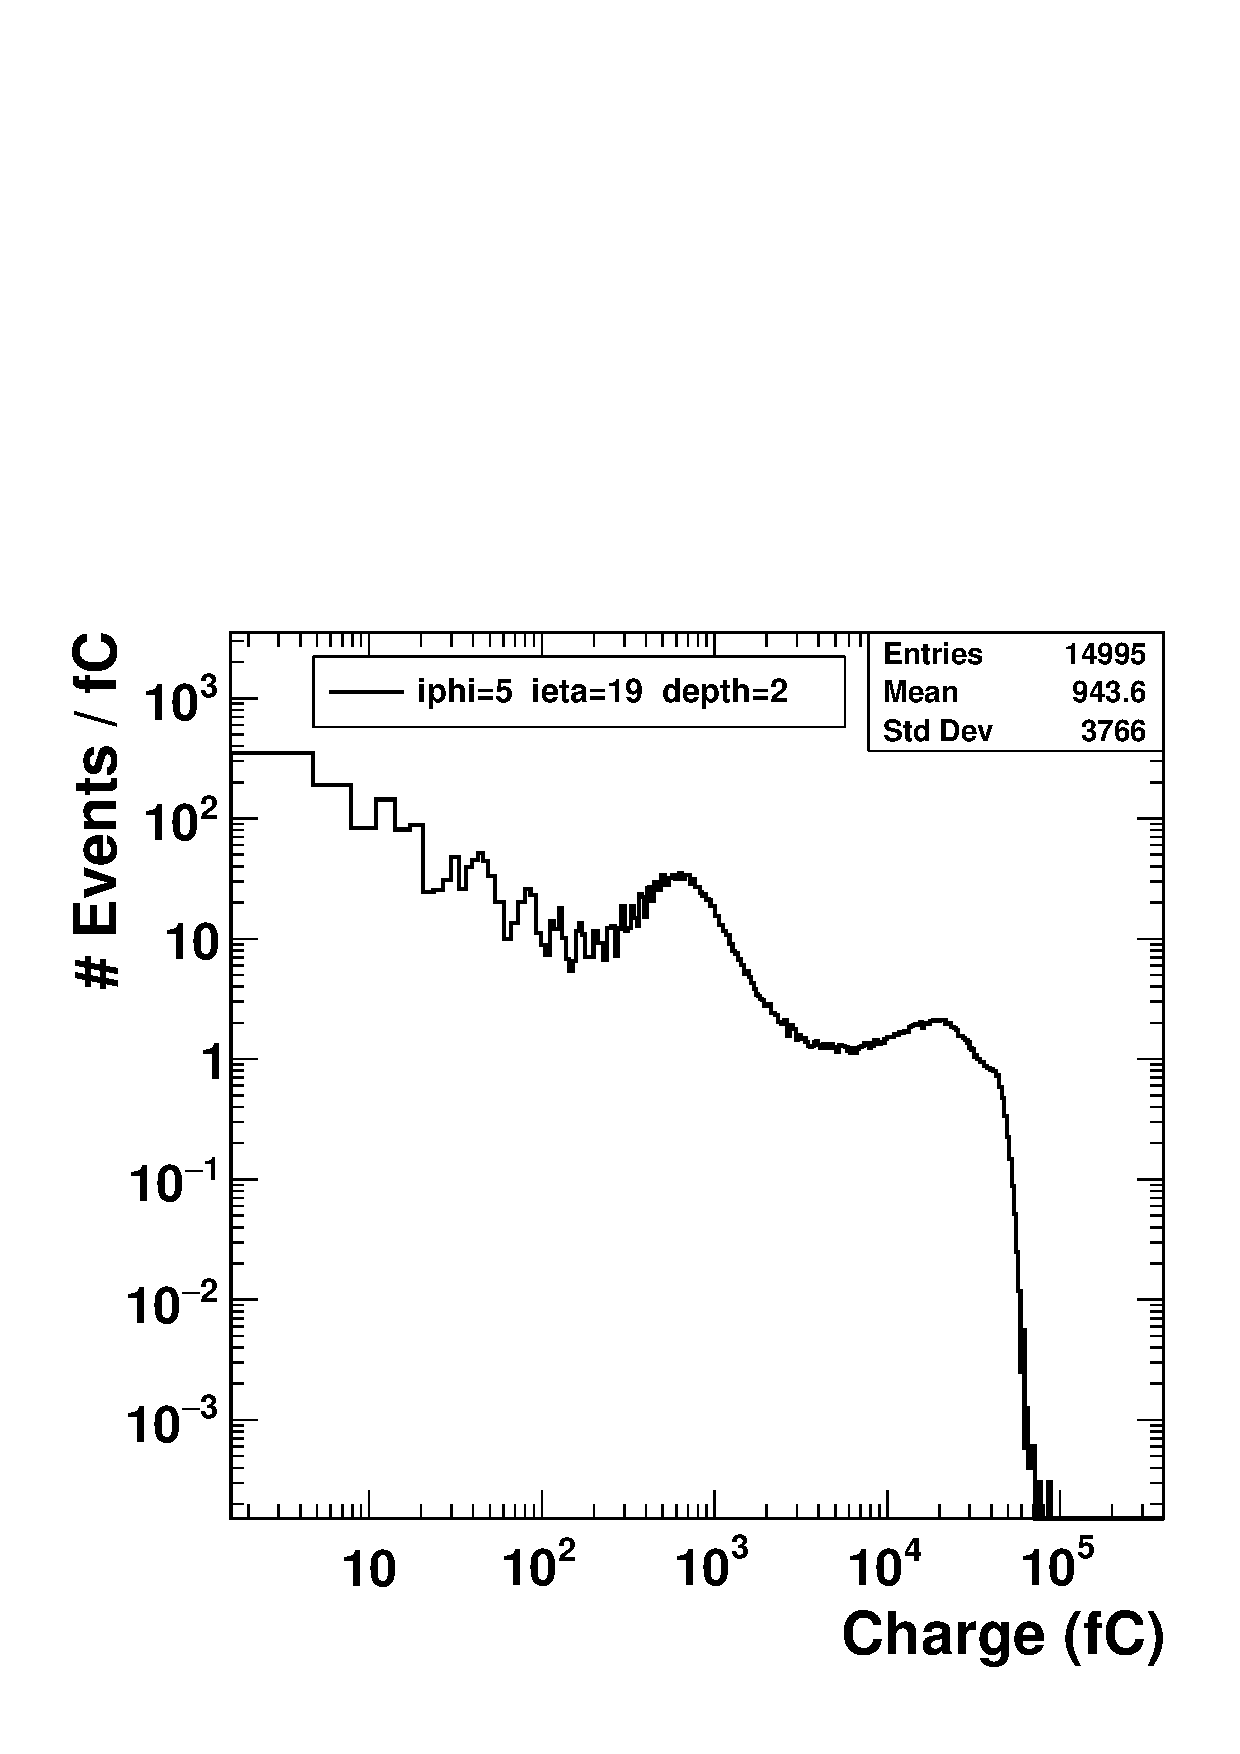
\includegraphics[width=0.7\linewidth]{Figures/pioncharge.pdf}
\caption{Charge distribution for a single channel (ieta=19, iphi=5, and depth=2) in a 50\GeV\space pion run aimed at ieta=19 and iphi=5. The peak on the right shows the average output charge in response to the incident particles at this energy.}
\label{fig:pioncharge}
\end{figure}

The output charge distributions in events with different incident pion energies are shown in Figure~\ref{fig:Log}, which shows the number of hits that output a certain charge. This figure can also be used to start the analysis on the SiPM nonlinearity. One key thing about the nonlinearity is that at low charge output and correspondingly low particle energy, the SiPM is expected to have a linear output, and only at high output charge does this effect become significant. This means that, in order to study nonlinearity, one needs to use particles at sufficiently high energies. Unfortunately the highest beam energy that can be achieved with the test beam yields a signal in the range in which the SiPM nonlinearity effect is only at a few percent. To illustrate this, by looking at Figure~\ref{fig:Log} it is apparent that in the $300\GeV$ run, an energy close to the maximum the test beam is capable of producing, there are minimally few events that output charge above 300,000 fC. The SiPM outputs approximately 40 fC for every incident photo electron, which means the highest energy events create about 6000 incident photo electrons. When using a simulation of the SiPM it is apparent that this is still very much in the linear range of the SiPM. One thing to note is that not all of a single particle's signal goes to a single SiPM. Figure~\ref{fig:pioncharge} shows that while the majority of the particle's energy is deposited in the first group of scintillator tiles it hits, there is still a significant portion in neighboring channels. Summing over all the channels should give the total energy of the particle, but this means that 300,000~fC does not directly translate to $300\GeV$. As the energy of the particle increases its energy will spread out more, which means a $600\GeV$ pion will not necessarily deposit 12,000 photo electrons in the first channel it hits.

\begin{figure}
\centering
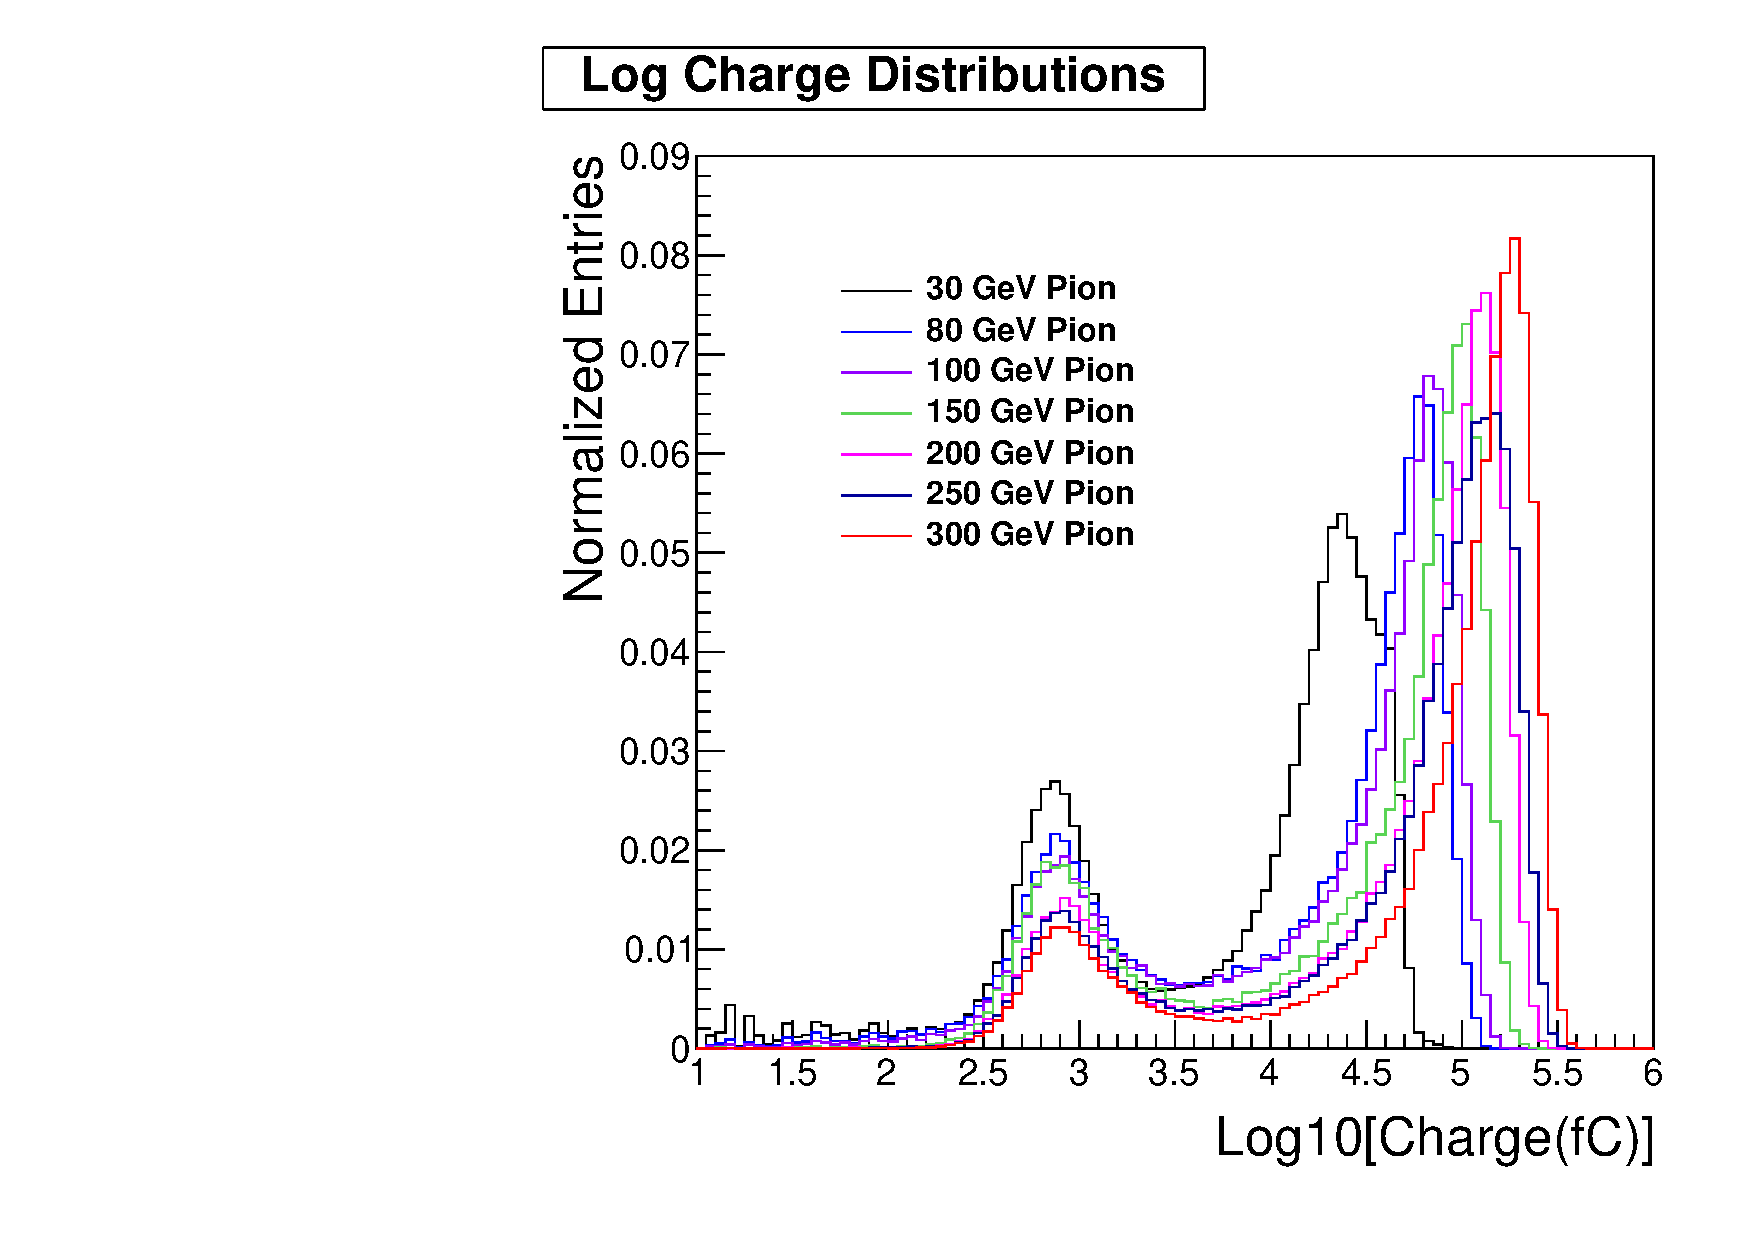
\includegraphics[width=0.7\linewidth]{Figures/Logplot.pdf}
\caption{Distributions of charge signals from the channel iphi=5, ieta=19, and depth=2 in events with different pion energies.}
\label{fig:Log}
\end{figure}

One of the key things in doing a pulse shape analysis using test beam data is the timing information. In the test beam, we have two different pieces of timing information. The first comes from the QIE chips in the readout modules. The readout modules measure the output charge of the SiPM over 250~ns, and the information is binned into 10 time samples each 25~ns long, which is shown in Figure~\ref{fig:PulSh}. The output pulse of the SiPM is about 75~ns long, and it usually stays confined to 3 or 4 time samples. In addition, we also record what is called a Time to Digital Converter (TDC) value. This value stores at what time in the 250~ns span the output charge of the SiPM crossed a threshold, with 0.5~ns resolution. Since the output charge starts out below this threshold, the TDC value should give the start of the output pulse of the SiPM. For instance, a TDC value of 20 in time sample 4 means that the pulse crossed the threshold charge value 10~ns after the start of time sample 4 or 110~ns after the start of data taking. One of the problems with the TDC value is that it could be affected by the amplitude of the output pulse as a high amplitude pulse will cross this threshold earlier. To extract the pulse shape we can take the difference of pulses with different TDC values. 

\begin{figure}
\centering
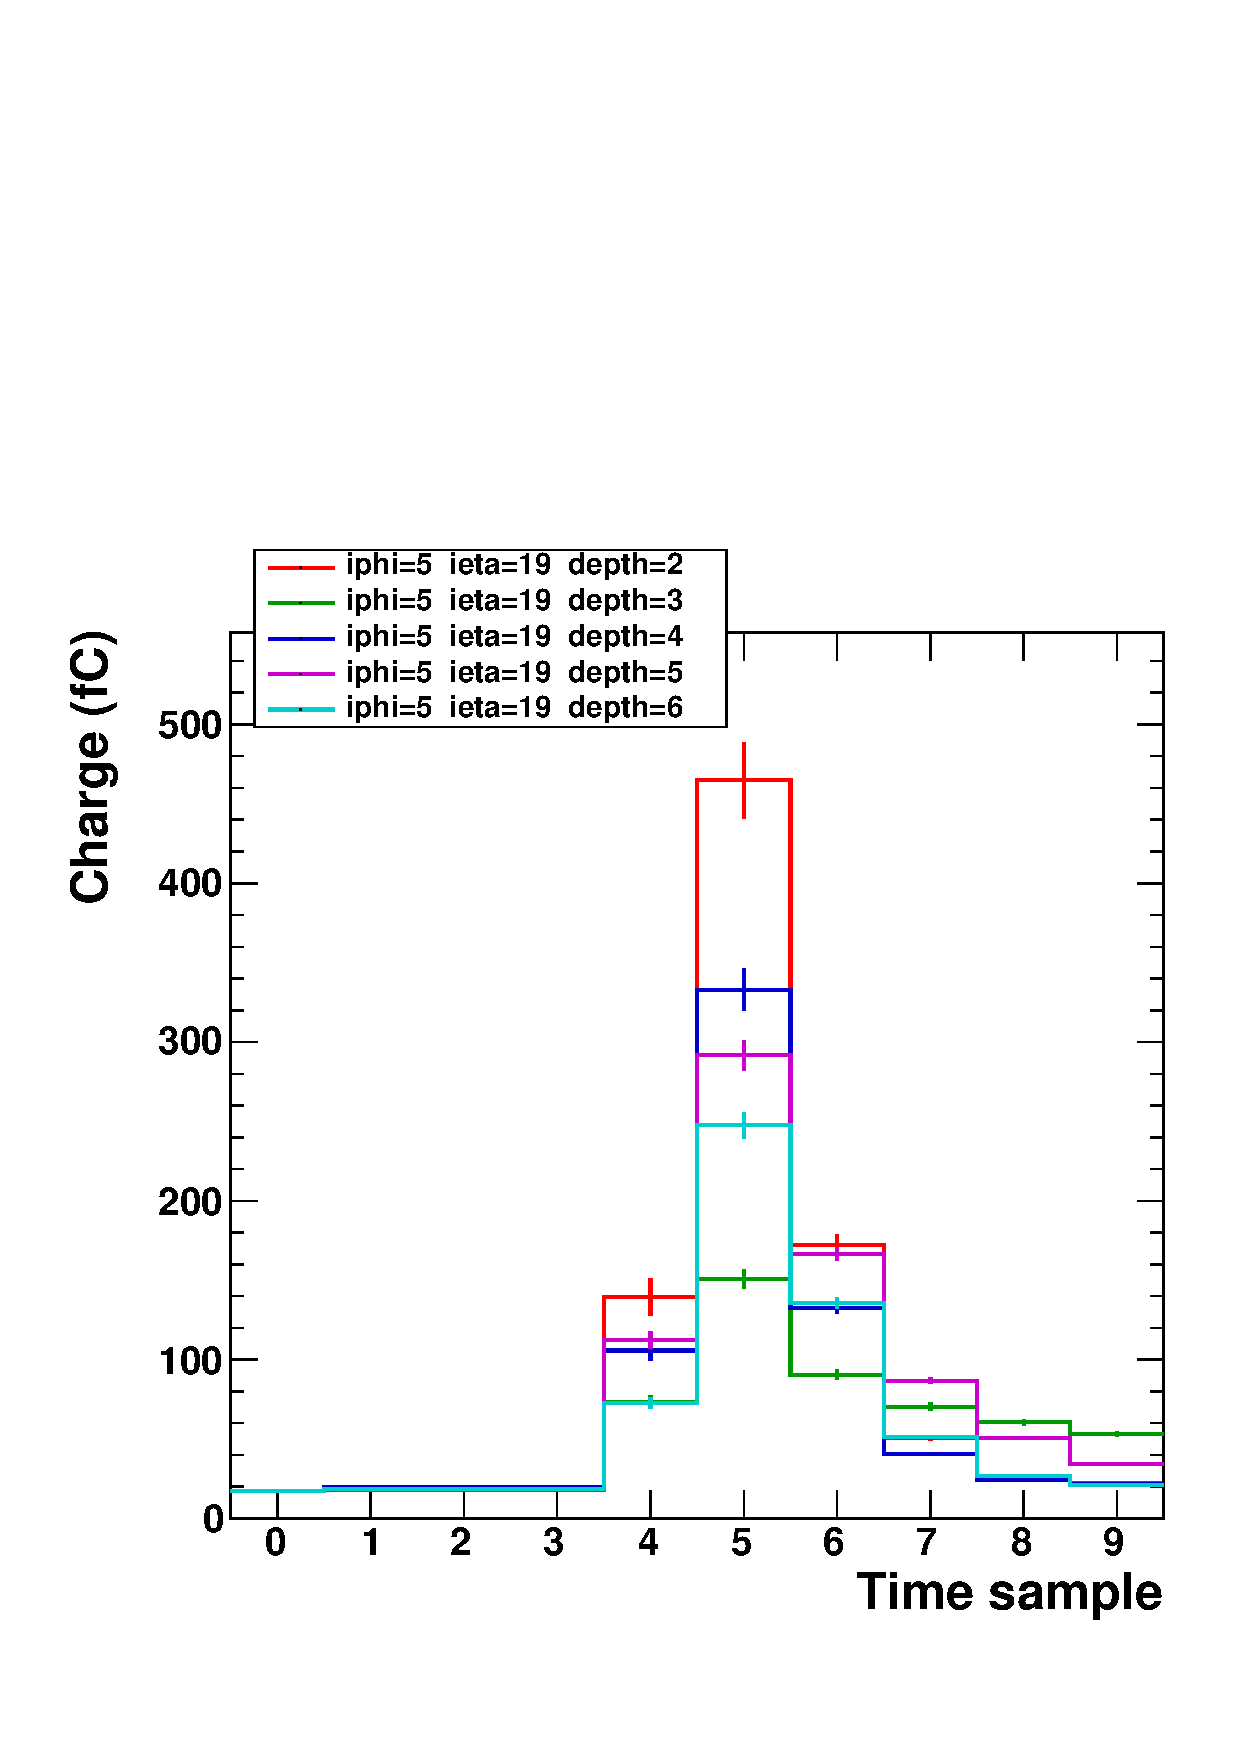
\includegraphics[width=0.6\linewidth]{Figures/Pulse.pdf}
\caption{The average output charge over time in ten time samples, each 25~ns long. This is from a run with 150\GeV\space muons aimed at iphi 5 and ieta 19. This plot shows the output pulse of the different depths at that location.}
\label{fig:PulSh}
\end{figure}

There is also timing information from the trigger system. The timing information from the trigger system does not have the amplitude dependence, which the TDC timing information may have; however, most people still use the TDC from the QIE chips. The relationship between the two signals can be shown in Figure~\ref{fig:tdc}. Theoretically, this timing information from the trigger system could be used to extract the pulse shape.

\begin{figure}
\centering
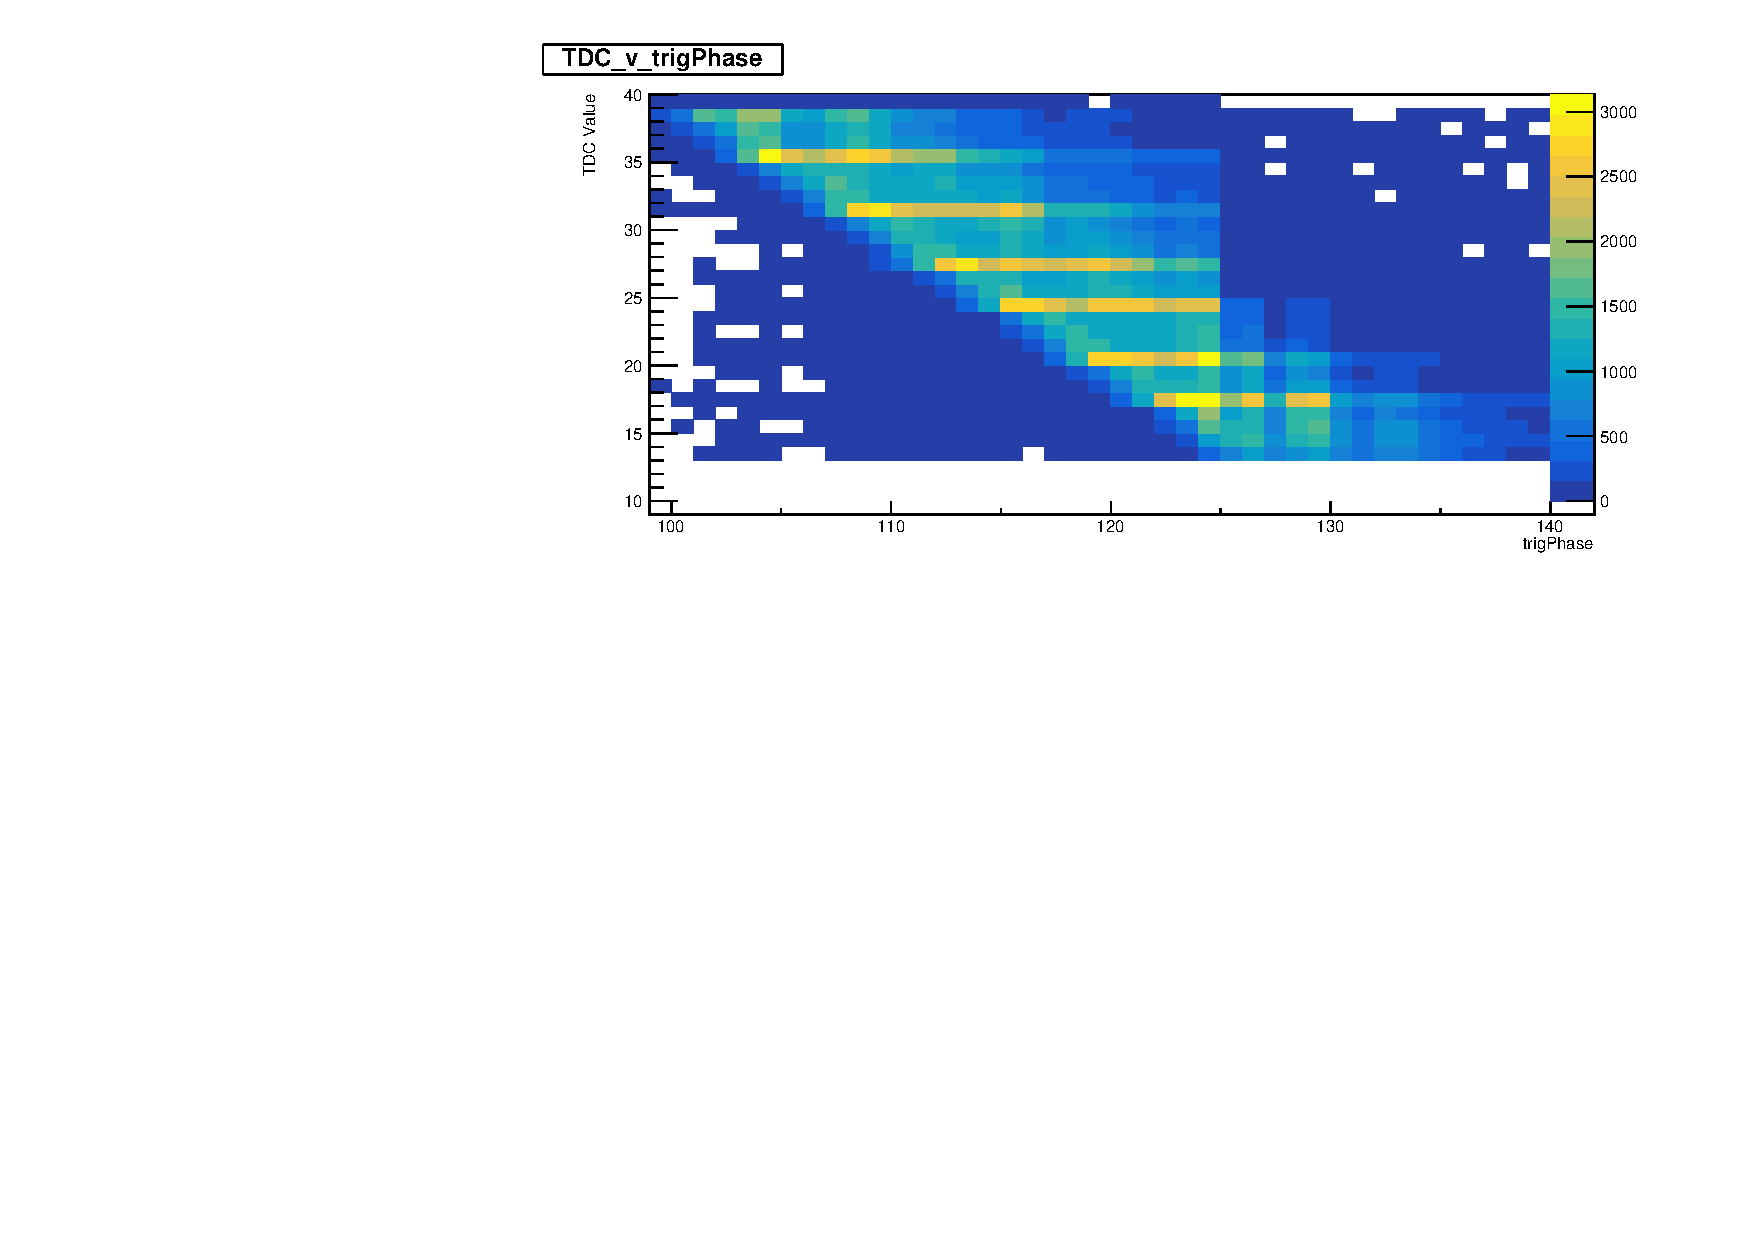
\includegraphics[width=\linewidth]{Figures/TDCvTrigPhase.pdf}
\caption{The correlation between the trigger timing information and the QIE TDC information.}
\label{fig:tdc}
\end{figure}

When we take a run using the test beam, we do not just take data from one single particle but several thousand stored in their own individual events. Because of the nature of the test beam, there is some randomness in the arrival time of the particles in the beam. When extracting the pulse shape, we use this randomness by looking at pulses with the same total charge but different TDC values. Theoretically, two pulses with the same charge but different TDC values should be exactly the same except for a time shift. These pulses could look different in data, however, as different parts of the pulse will be put into different time samples. Figure~\ref{fig:bin} shows an analog pulse shape along with its binned output. In our analysis method, to extract the pulse shape, we take the difference in binned pulse value from several different pulses, all with similar overall charge but with a range of TDC values. Figure~\ref{fig:Phase} shows multiple sets of data, all with different TDC values, illustrating how changing the TDC value can change the bins without changing the total output charge. An example of this is taking the difference in the charge value from time sample 4 in a pulse with a TDC value of 20 and the charge value from time sample 4 in a pulse with a TDC value of 21 gives the pulse height at 110~ns in the 250~ns long data set. Doing this process over all the time samples with more pulses and TDC values ranging from 0--49 in time sample 4 will give a more analog version of the pulse shape shown in Figure~\ref{fig:fit}.

\begin{figure}
\centering
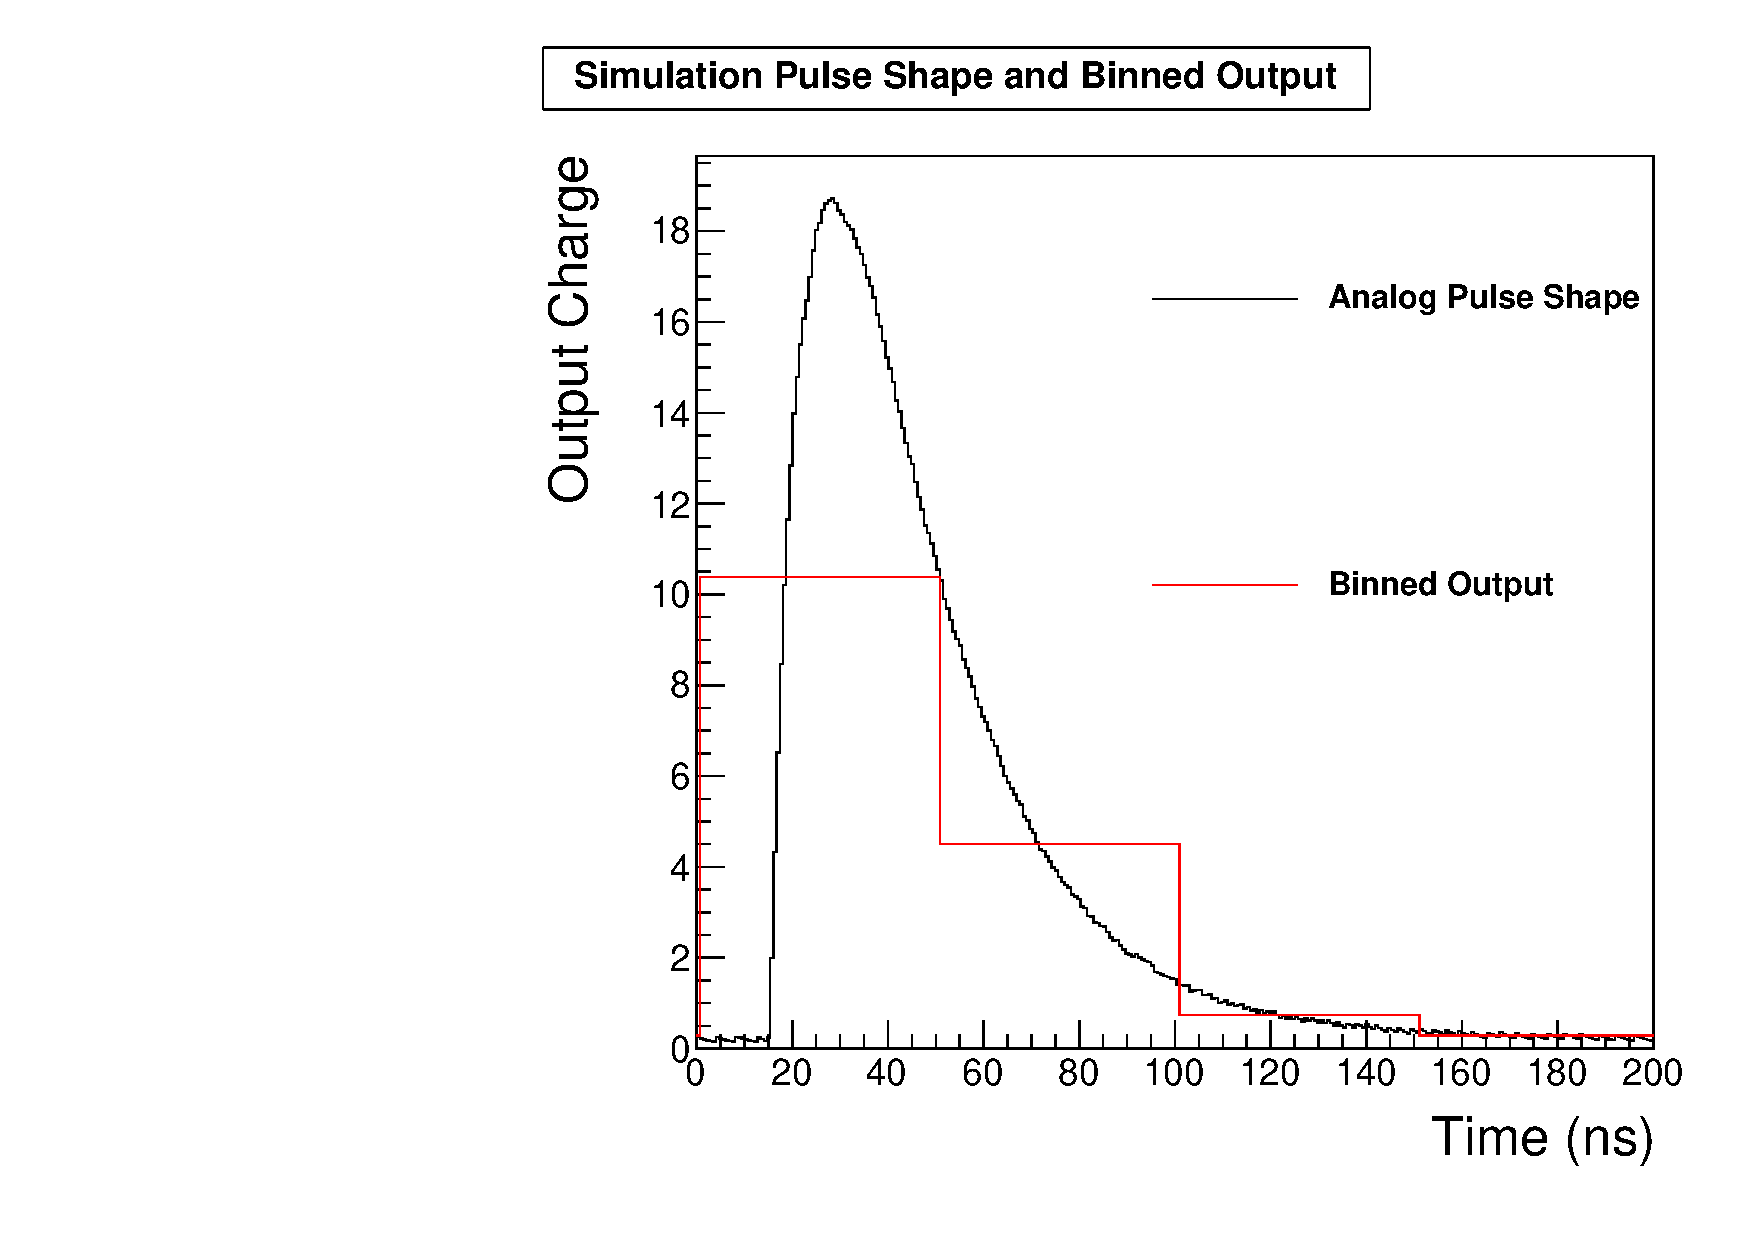
\includegraphics[width=0.6\linewidth]{Figures/Bin.pdf}
\caption{A SiPM simulation showing an analog version of the output charge along with the same output binned into time samples of 25~ns.}
\label{fig:bin}
\end{figure}

\begin{figure}
\centering
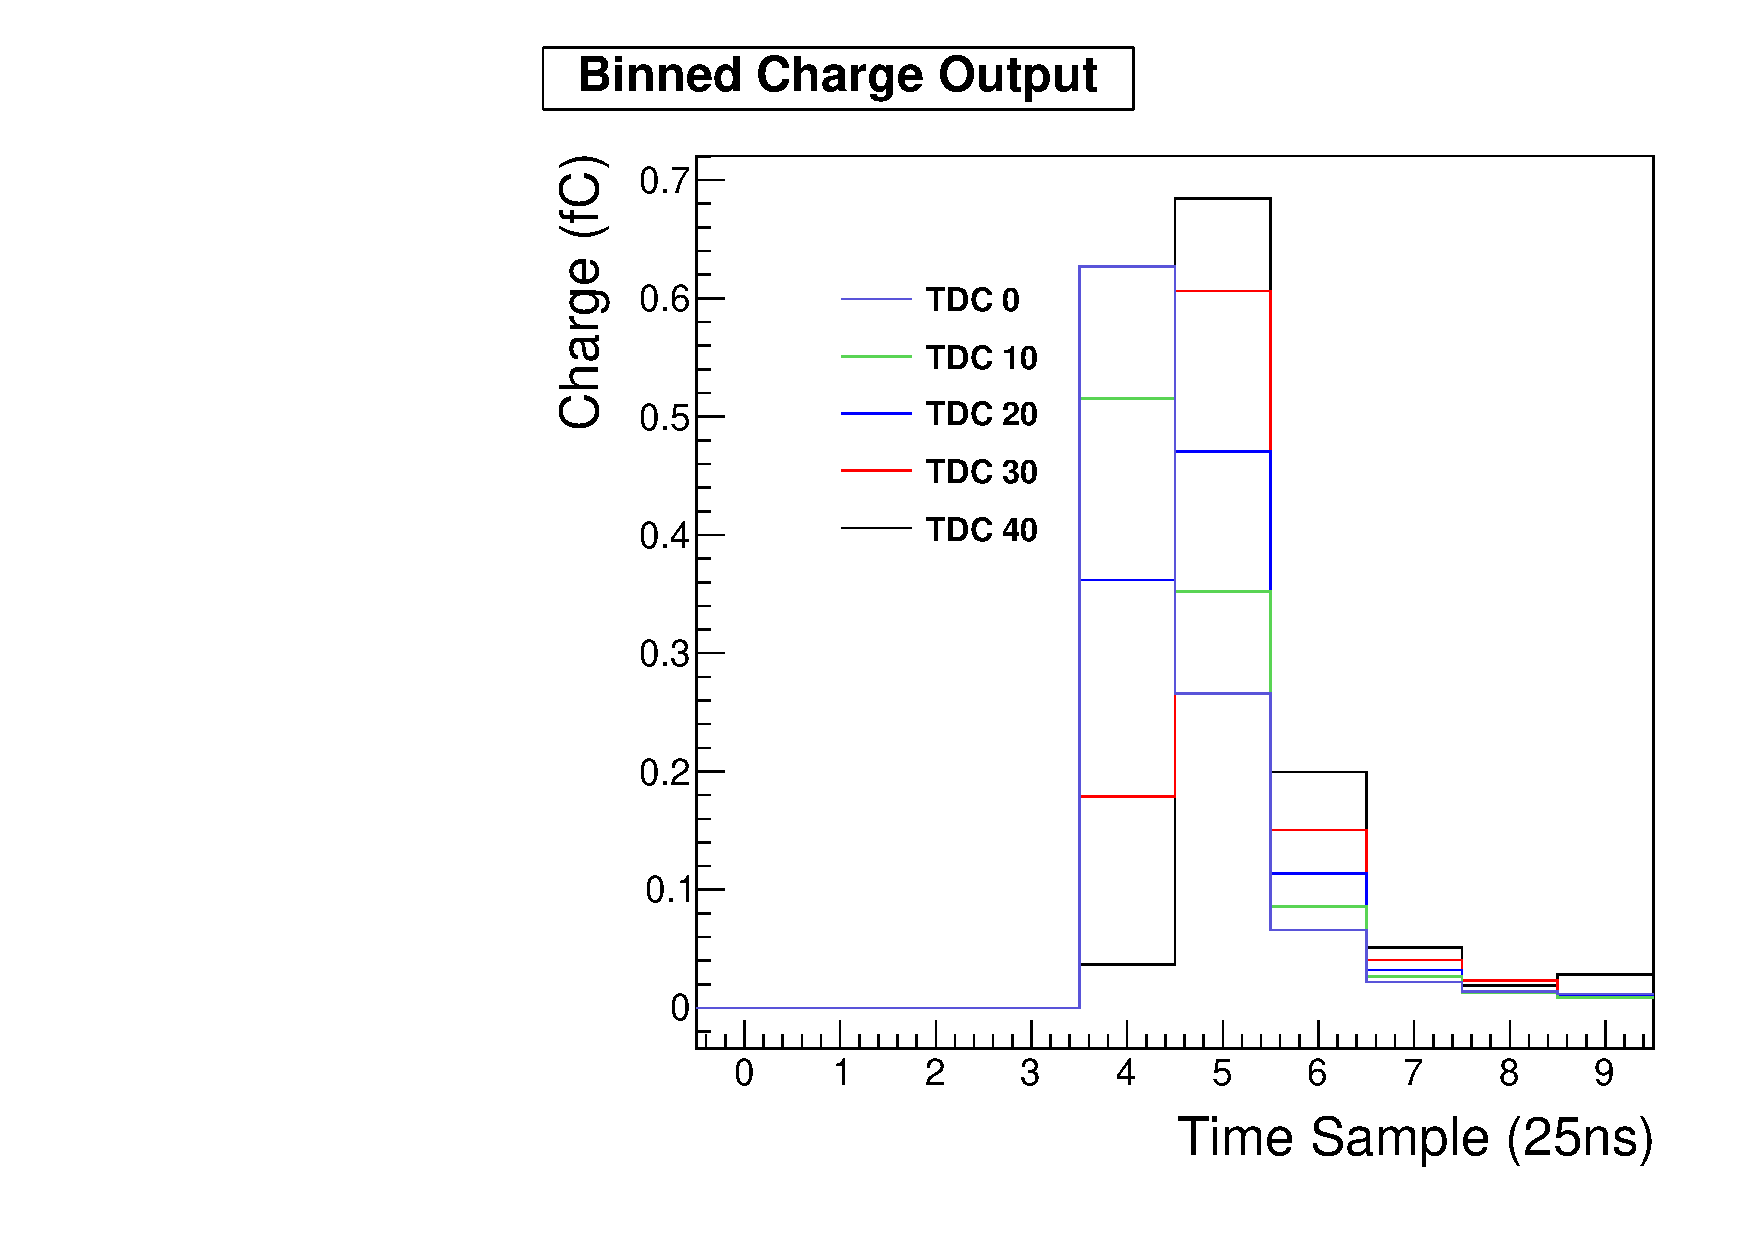
\includegraphics[width=0.6\linewidth]{Figures/Phase.pdf}
\caption{The binned output charge of events with different TDC values. All pulses have their TDC value in time sample 4 and have a total output charge in the range of 50,000--80,000 fC.}
\label{fig:Phase}
\end{figure}

\begin{figure}
\centering
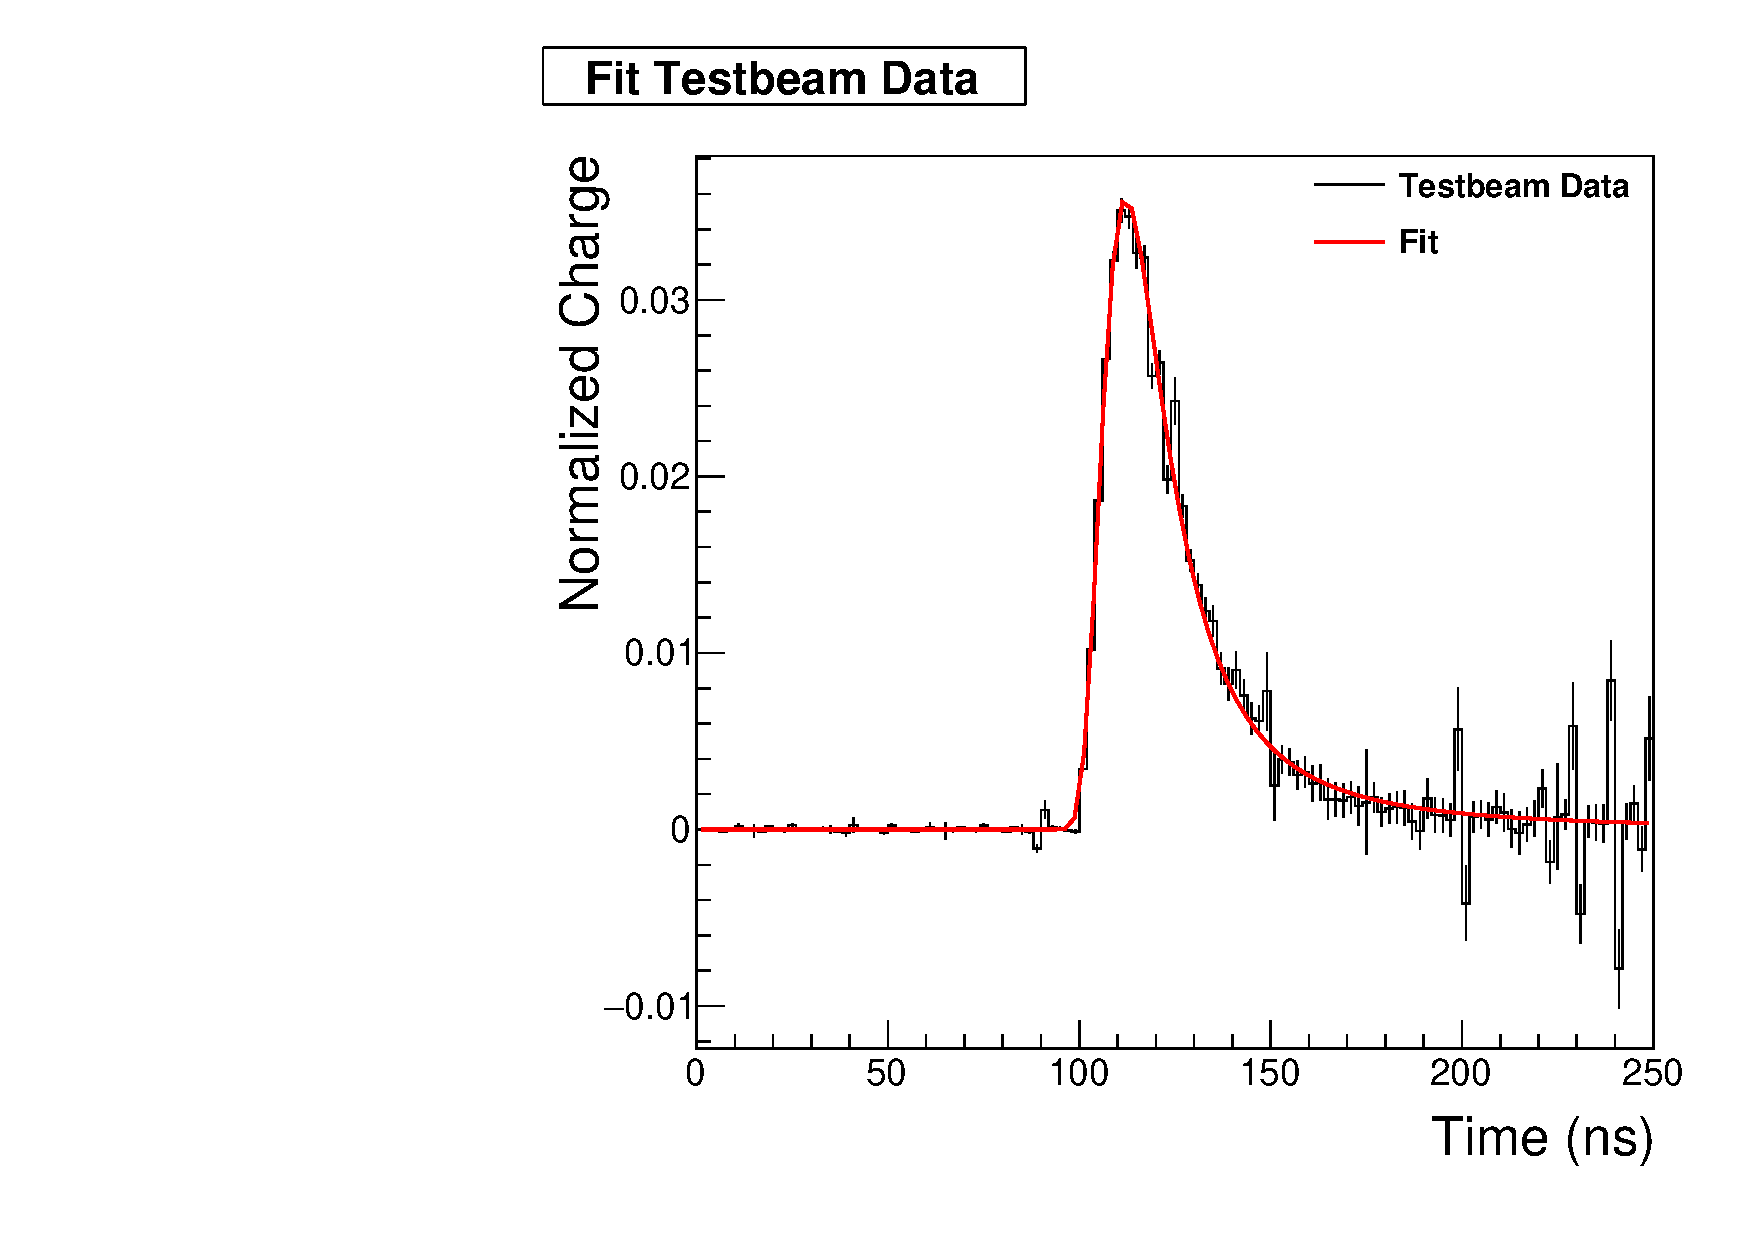
\includegraphics[width=0.6\linewidth]{Figures/FittedPlot.pdf}
\caption{A more analog version of the SiPM pulse shape obtained from test beam data. It is also fit to a Landau-Gaussian function. The total output charge of signals used to extract this pulse shapes ranges from 10,000 to 29,000 fC.}
\label{fig:fit}
\end{figure}


When we extract the pulse shape from test beam data, we use events that have similar output charge. There are a variety of reasons for this, but one of them is that there is evidence that the pulse shape changes with output charge. To study this, we measure the pulse shape using events with different output charge and see if there are any significant changes. Although most of the particles will have an energy identical to the beam energy, it is common to have outliers. To minimize this disturbance we take events from several different runs with particle energies ranging all the way from $30 \GeV$ to $300 \GeV$ and collect together the events in which the output charge falls in a certain charge range. Figure~\ref{fig:fit_together} shows pulse shapes obtained from several different charge ranges. Figure~\ref{fig:Overlap} shows the fits of these pulse shapes superimposed for comparison purposes. These fits show that there is little change in the pulse shape as the charge increases, but there is a small trend visible in this plot. Looking at the peak of the pulses it is apparent that the lower charge pulses have lower peak heights. This lack of area is made up in the second half of the pulse as the lower charge pulses are slightly higher there, though this is harder to see as it is over a longer period of time. This result is not unexpected as the nonlinearity of the SiPM can shift the charge of the pulse towards the front. 


\begin{figure}
\centering
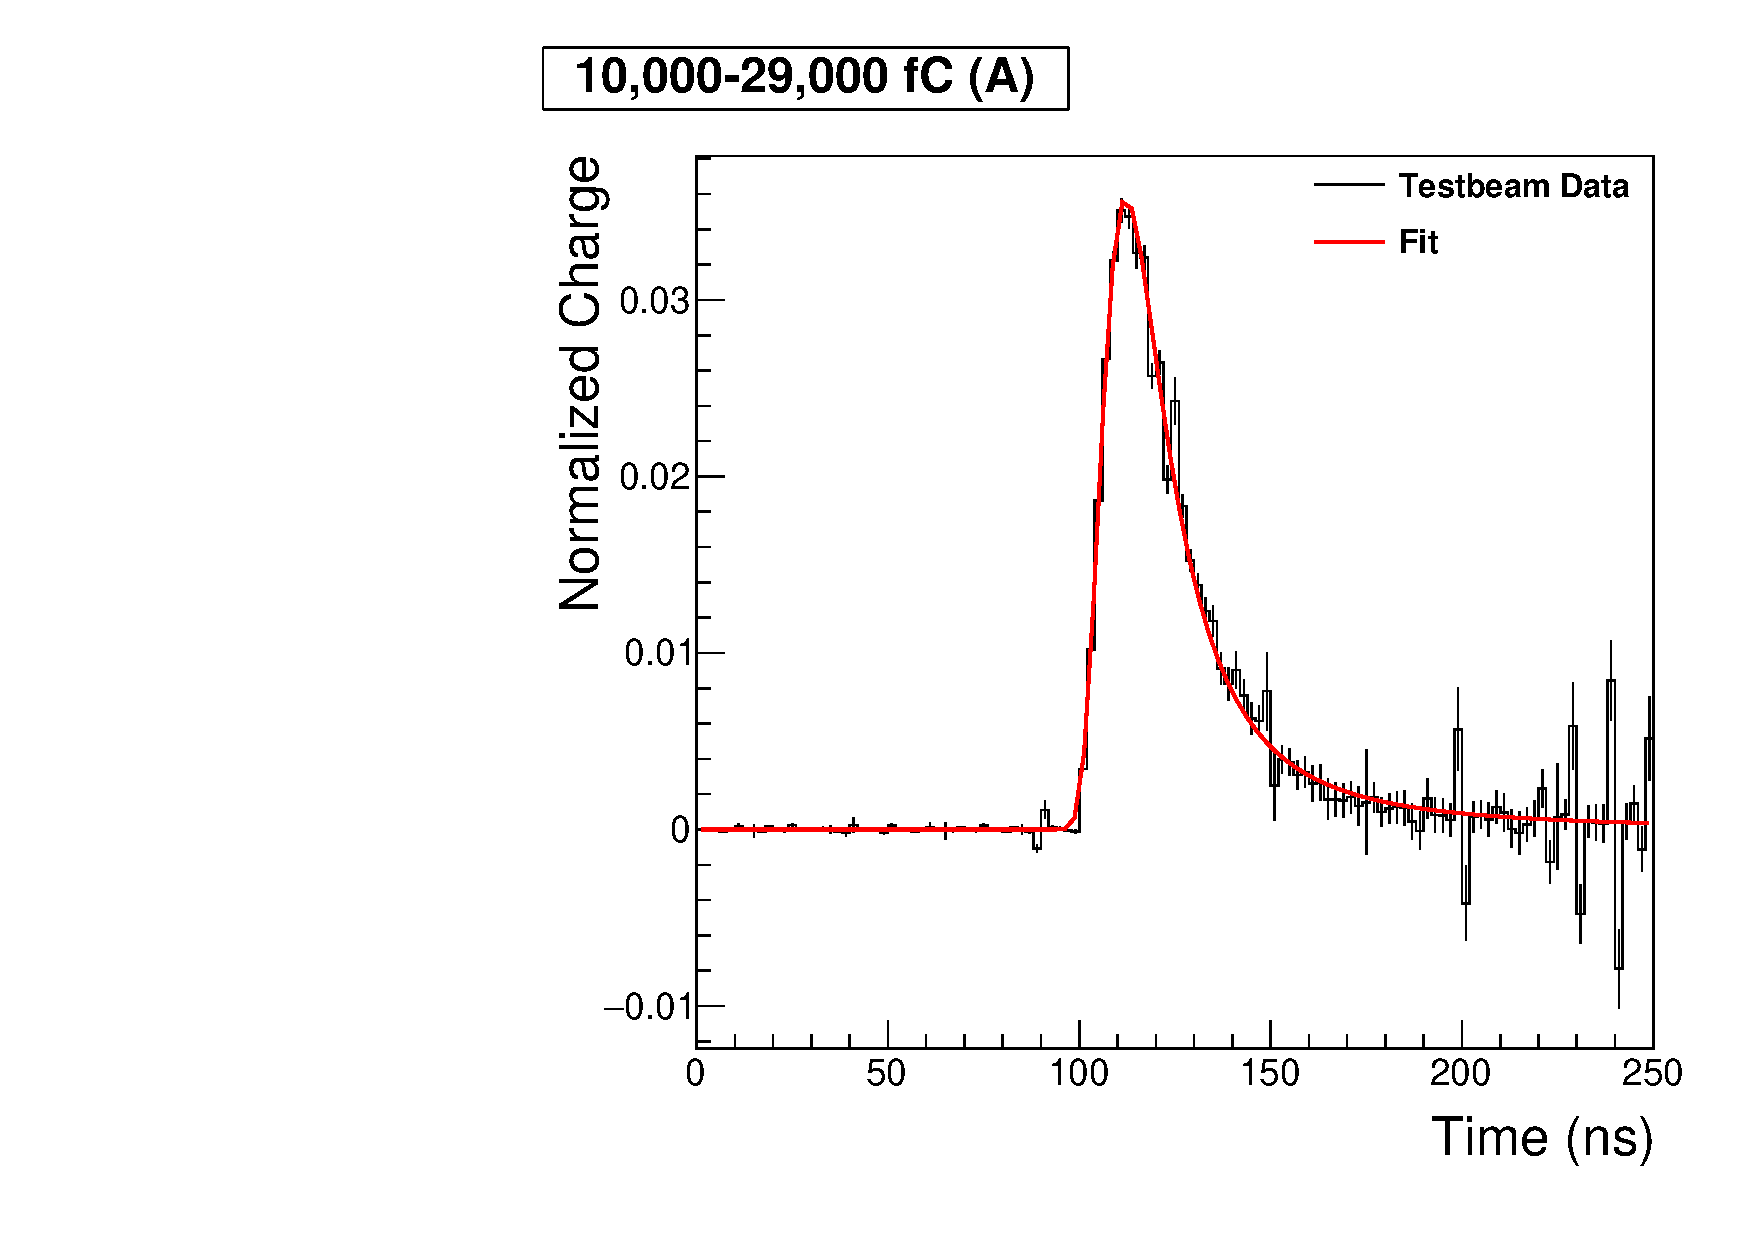
\includegraphics[width=0.4\linewidth]{Figures/10FittedPlot.pdf}
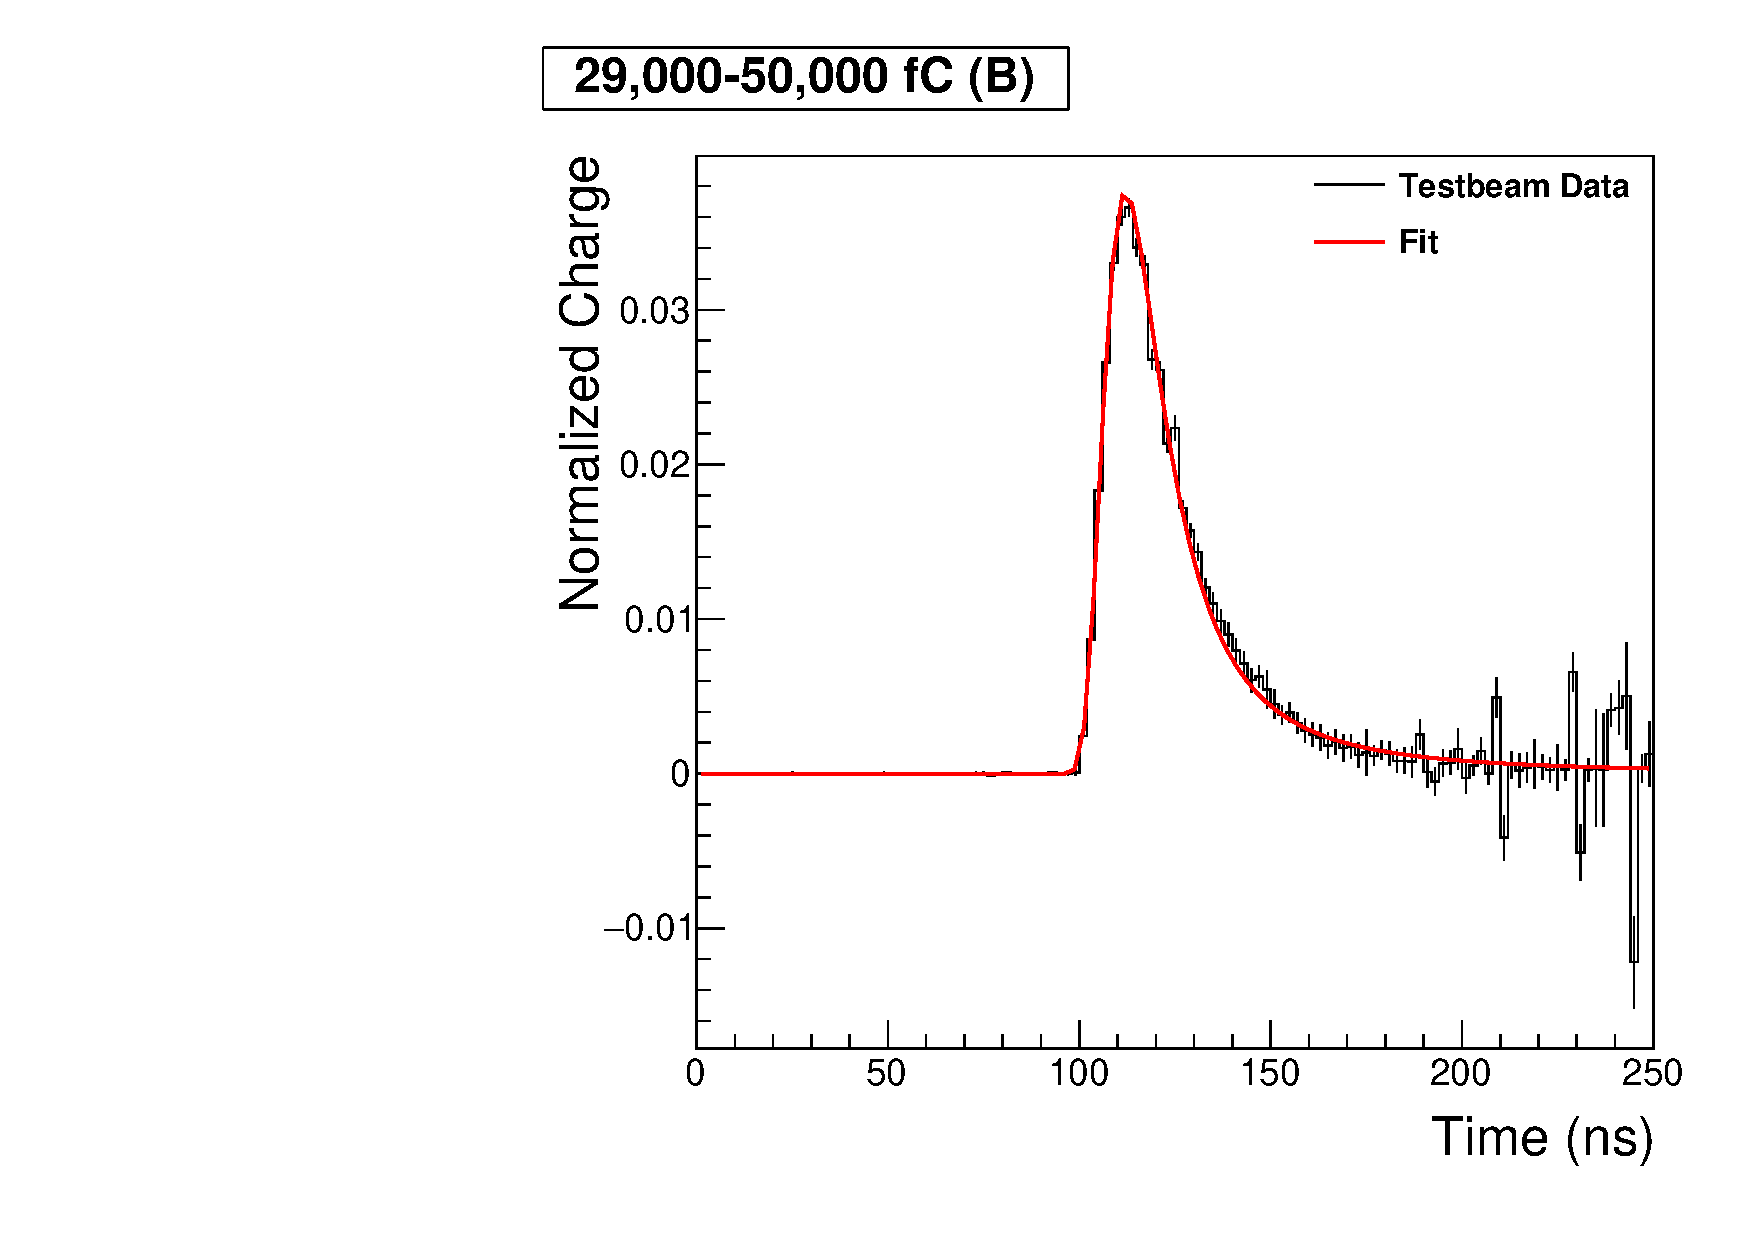
\includegraphics[width=0.4\linewidth]{Figures/29FittedPlot.pdf}
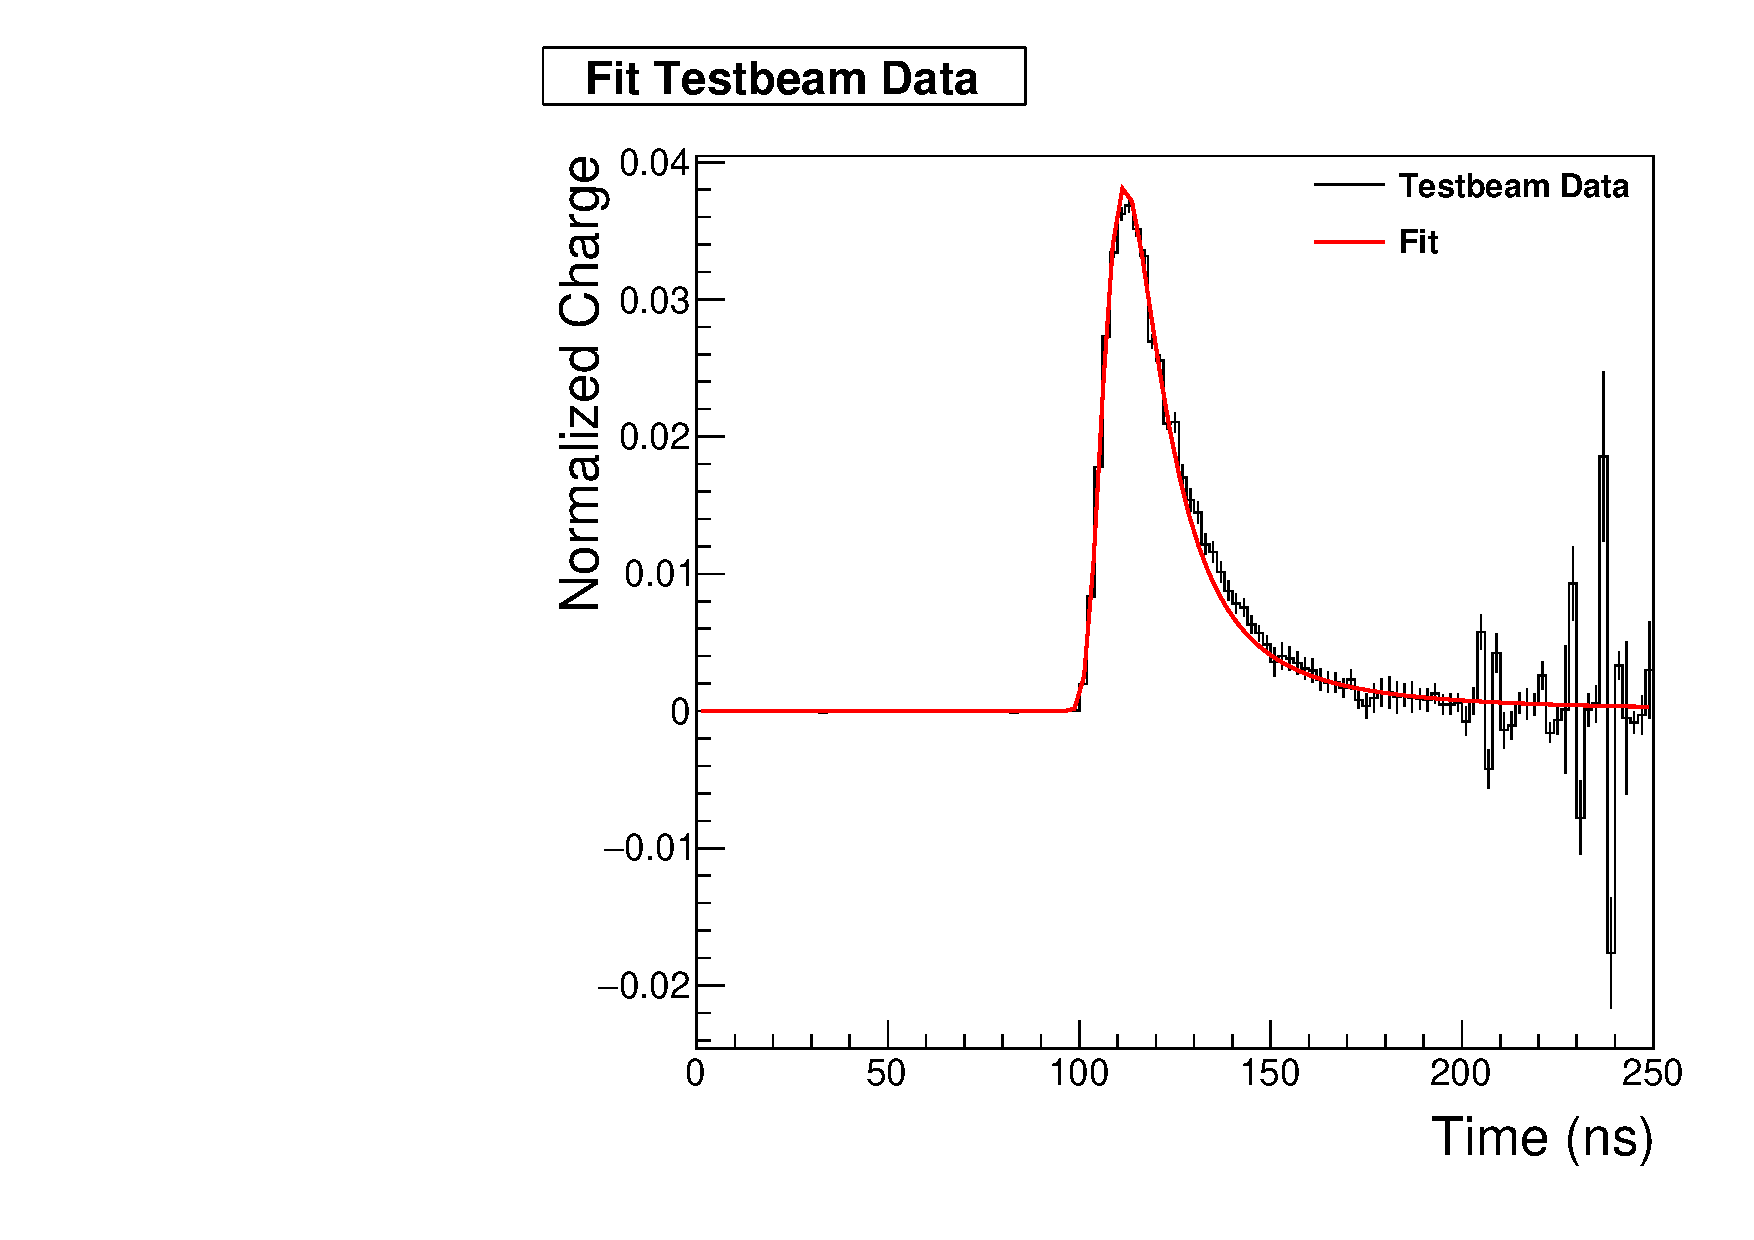
\includegraphics[width=0.4\linewidth]{Figures/50FittedPlot.pdf}
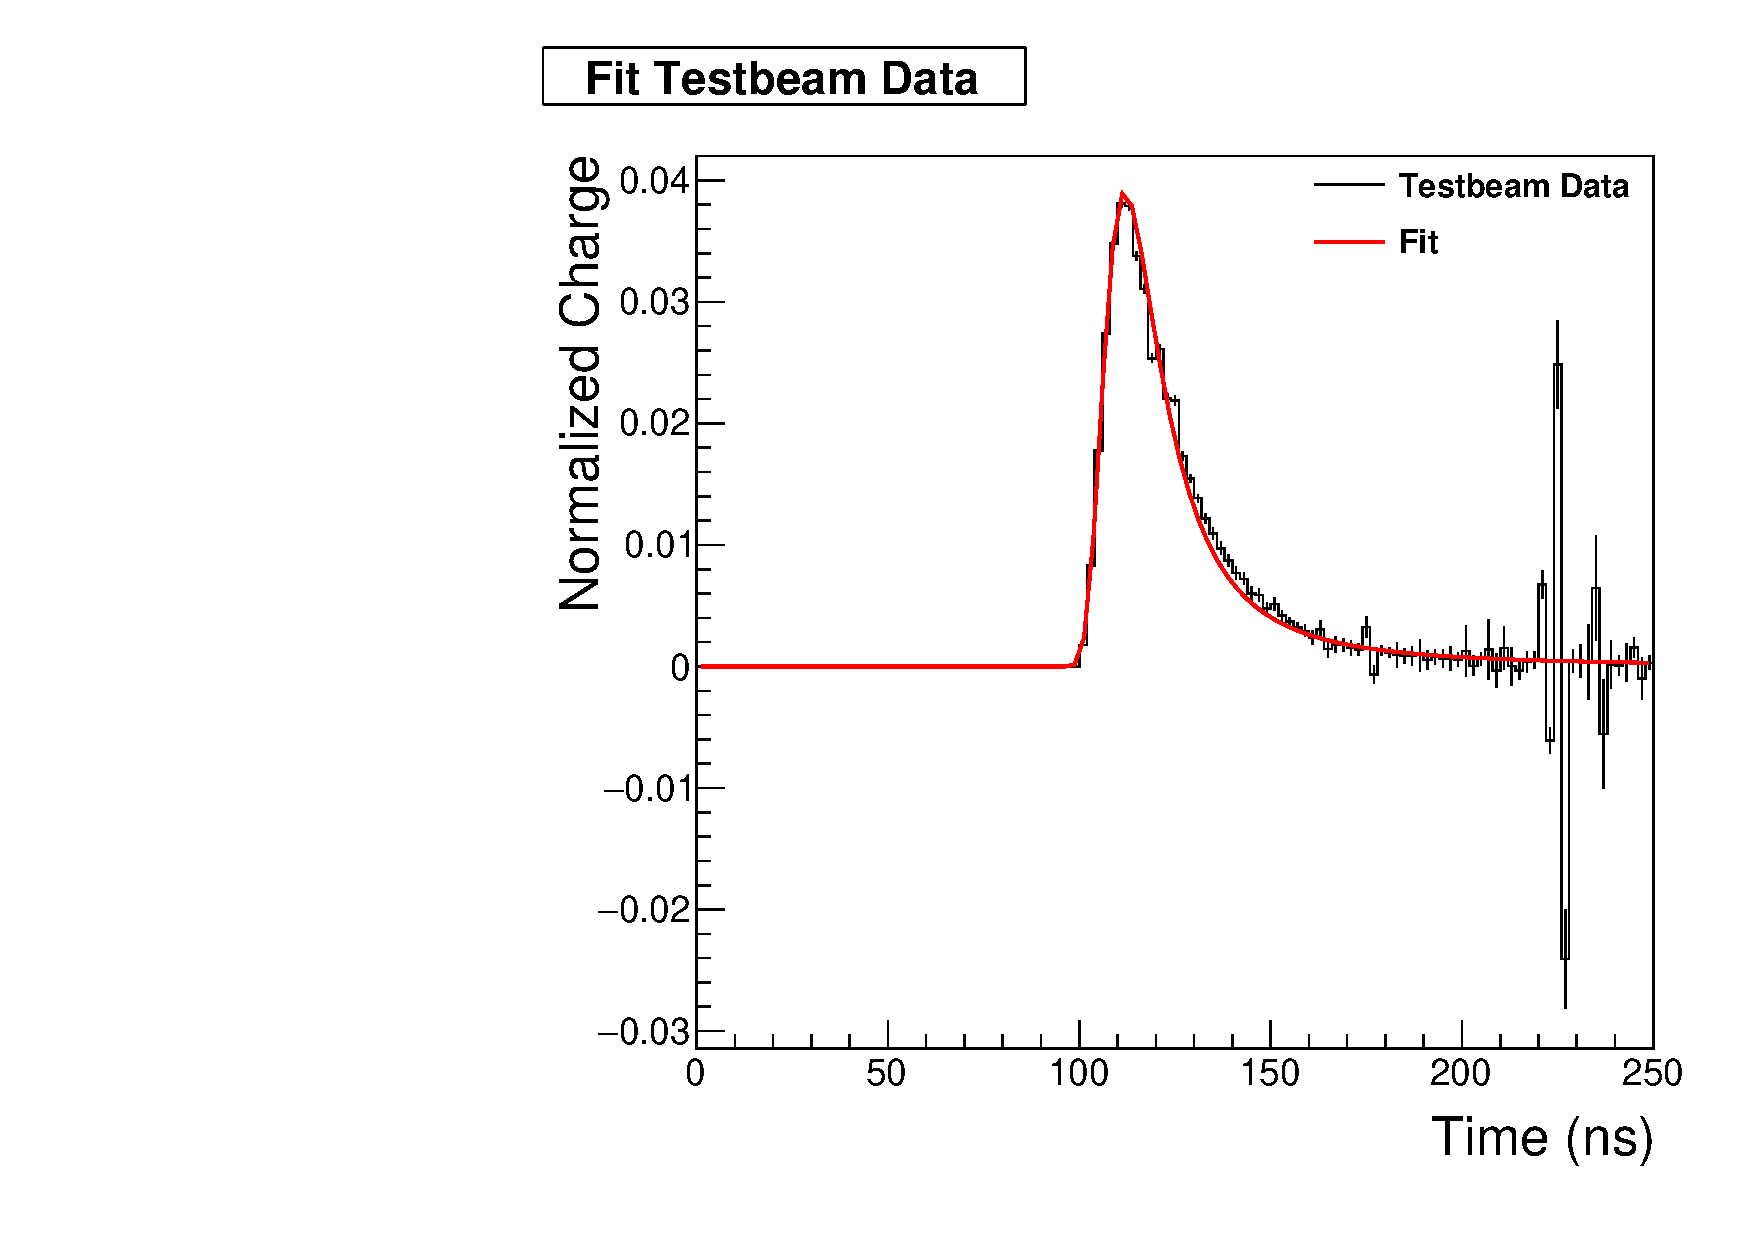
\includegraphics[width=0.4\linewidth]{Figures/80FittedPlot.pdf}
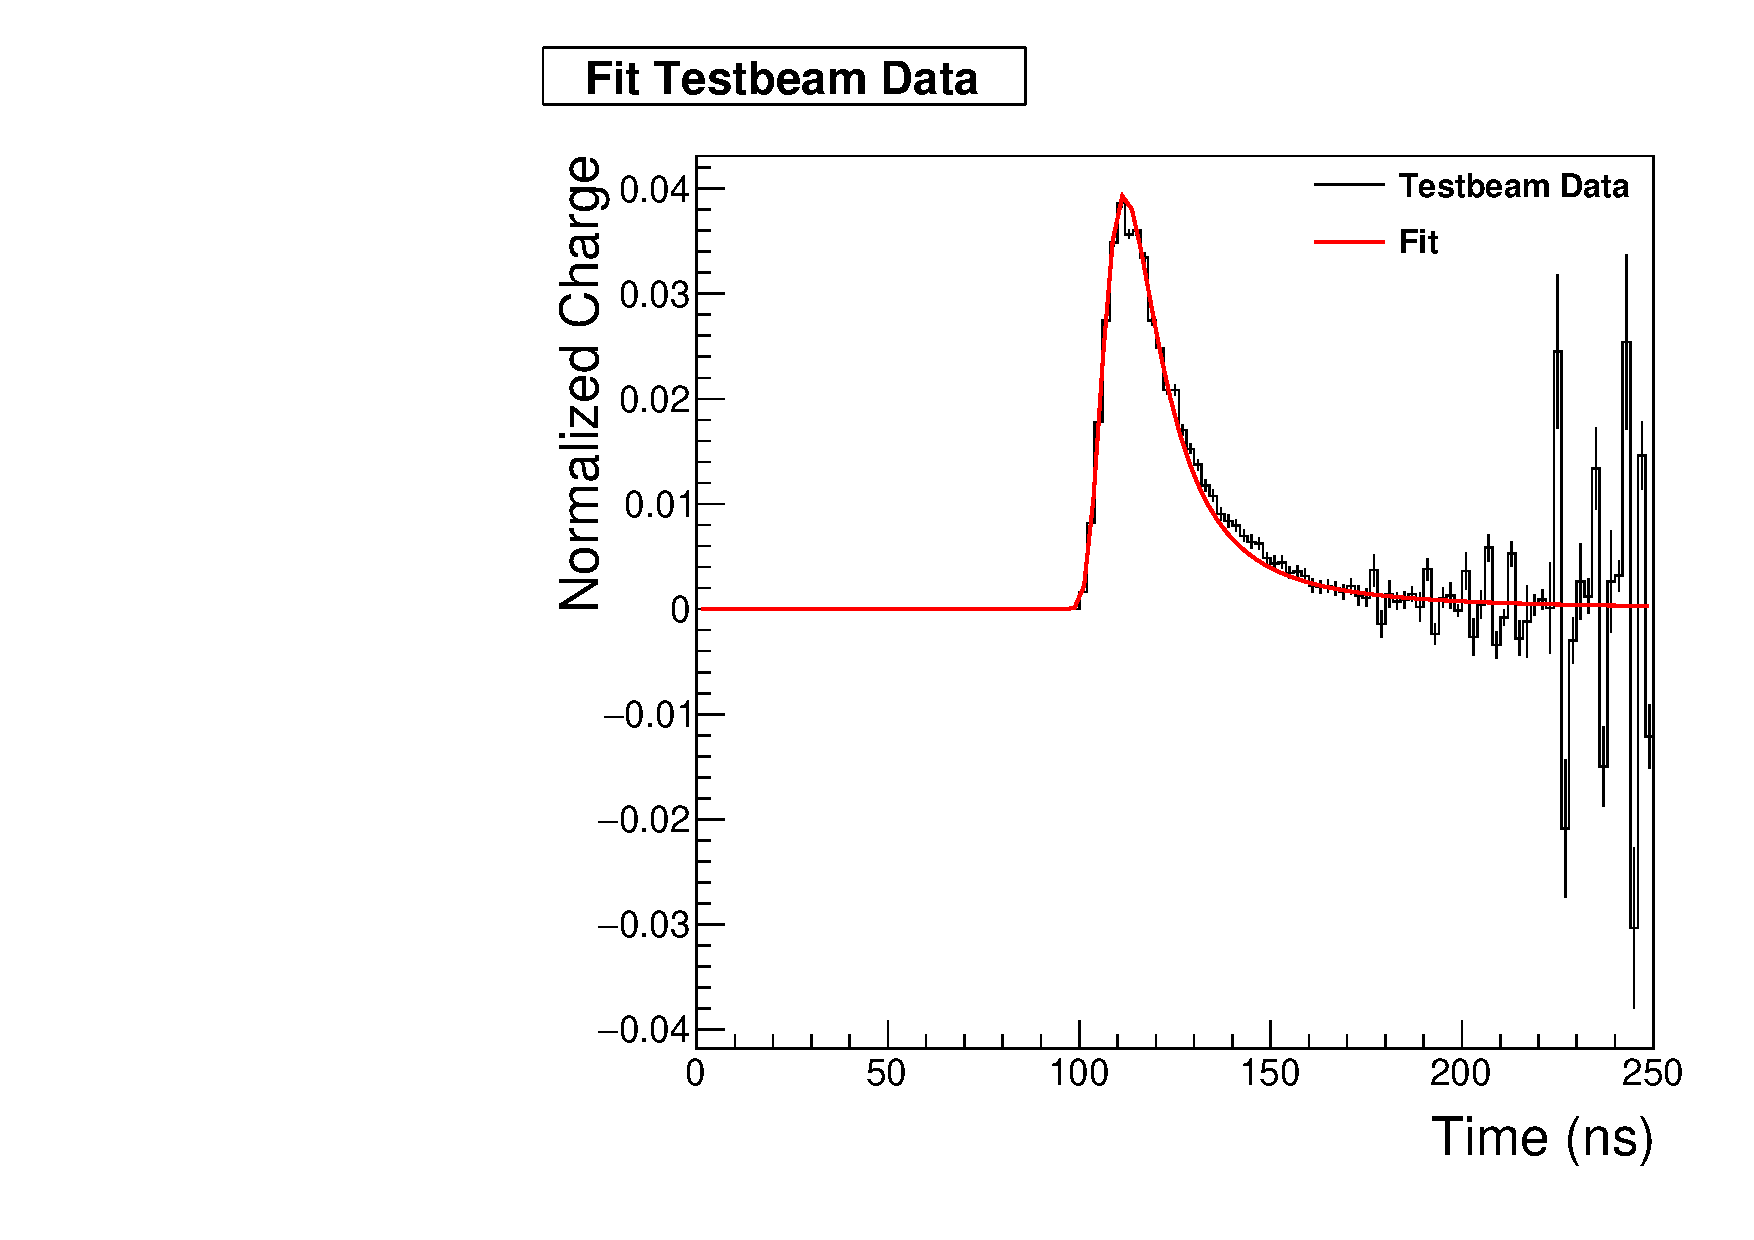
\includegraphics[width=0.4\linewidth]{Figures/125FittedPlot.pdf}
\caption{Fitted pulse shapes for signals in the charge range 10,000--29,000 fC (A), 29,000--50,000 fC (B), 50,000--80,000 fC (C), 80,000--125,000 fC (D), and 125,000--168,000 fC (E).}
\label{fig:fit_together}
\end{figure}

\begin{figure}
\centering
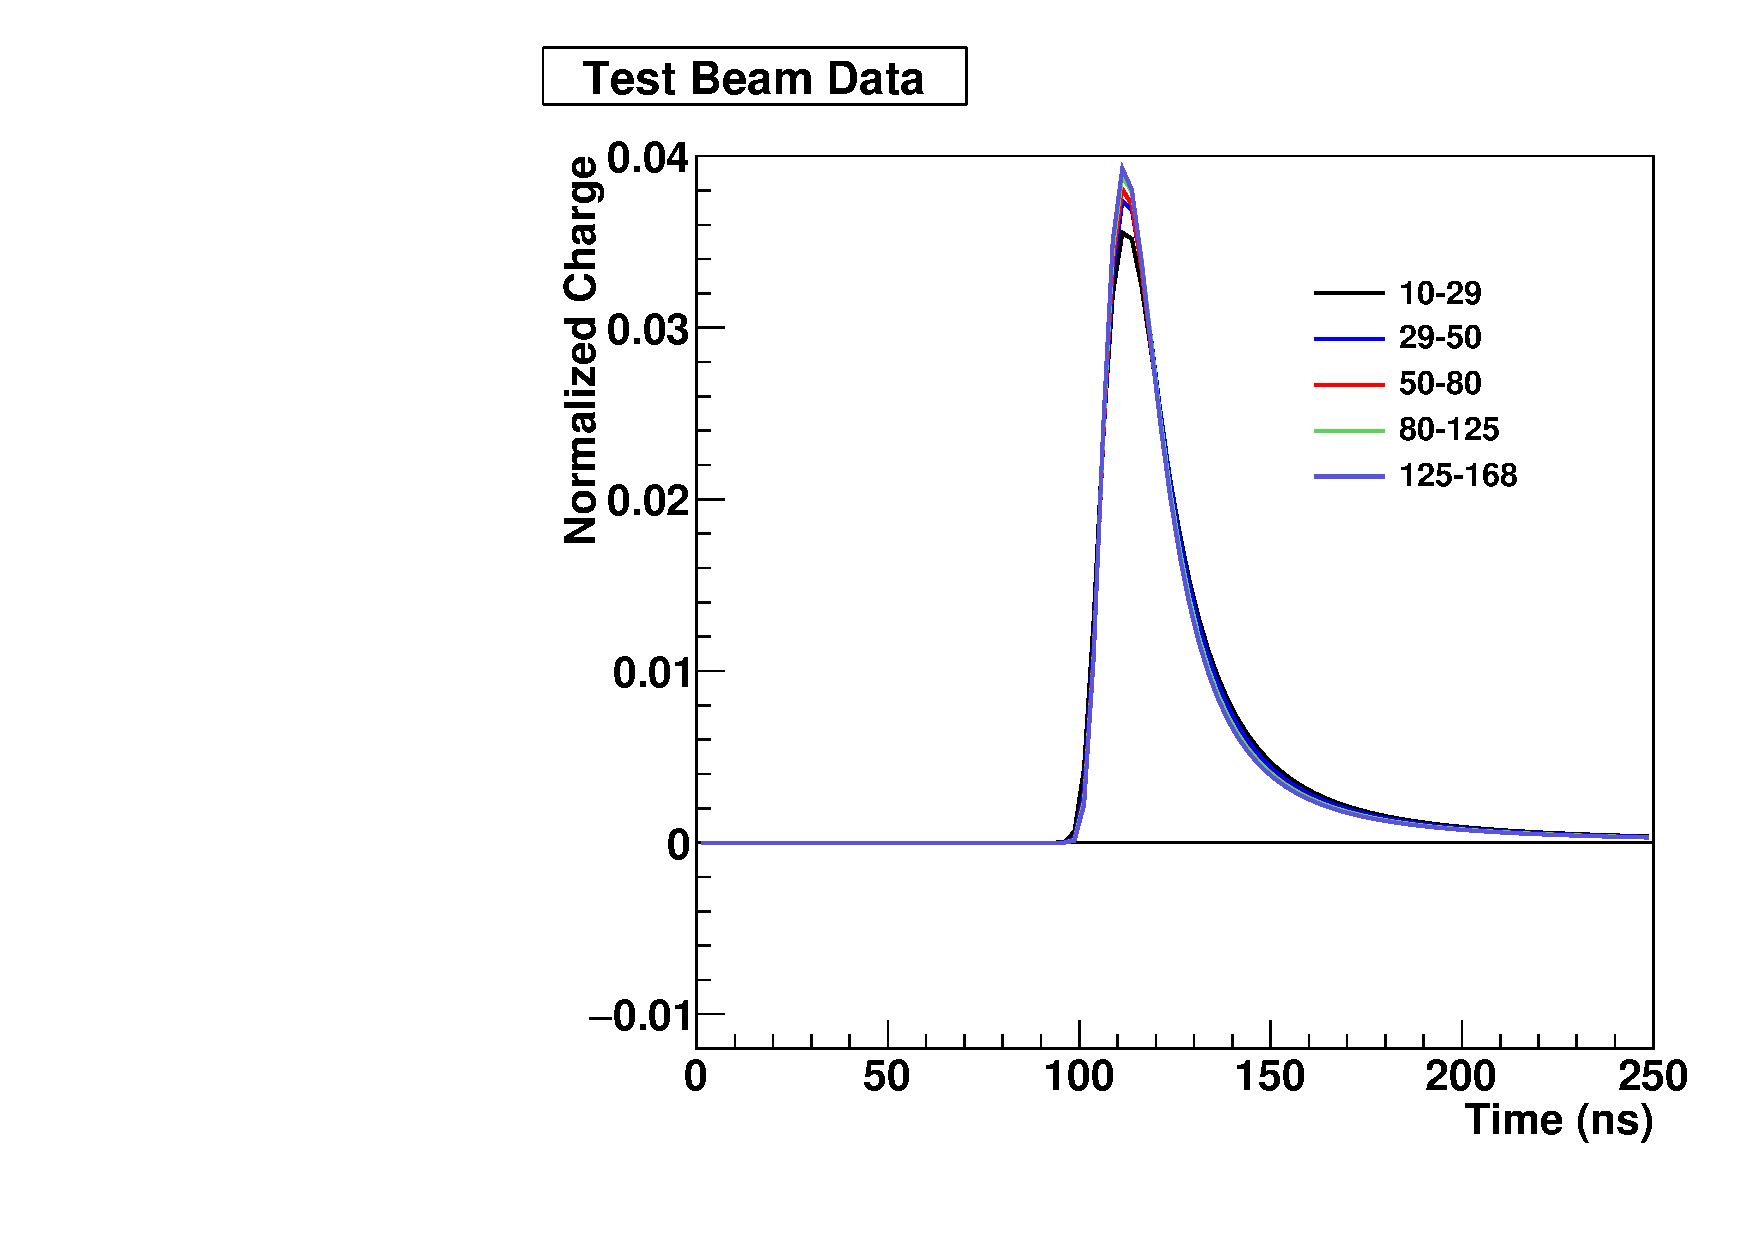
\includegraphics[width=0.8\linewidth]{Figures/Overlap.pdf}
\caption{Comparison of fits to pulse shapes obtained from different charge ranges.}
\label{fig:Overlap}
\end{figure}


\section{Summary}

Using test beam data, we were able to extract a precise pulse shape of the new readout modules. This pulse shape does appear close to expectations and has a reasonable fit to the Landau-Gaussian function. The pulse shape does show minor changes with changes in the output charge but at the energies from the test beam there were very little changes. The nonlinearity of the SiPM was not able to be studied in depth using the test beam data, but we were able to confirm that at energies from the test beam the SiPMs are very close to linear. These readout modules were installed in the HE on the CMS detector over the winter of 2018. 

